\chapter{Eigenvalues and Eigenvectors}
\label{chap:eigen}

In this section, we will discuss a very important topic in Linear Algebra, the \textit{eigenvalue-eigenvector} problem. By finding the eigenvectors of a square matrix that span subspaces that are \textit{invariant} under the corresponding linear operator, it is sometimes possible to obtain a coordinate basis such that the matrix can be \textit{diagonalized}, i.e.\ become a diagonal matrix under that particular change of coordinates. One of the practical usages of \textit{diagonalization} is to solve systems of linear \textit{ordinary differential equations (ODEs)} which are also commonly seen in many areas of Earth Science, such as chains of chemical reactions in the atmosphere. Moreover, many Earth Science applications suggested in the later chapters (e.g.\ Principal Component Analysis in Chapter \ref{chap:quad}, can be applied to seismic patterns) also depend heavily on the concepts of eigenvalues and eigenvectors.

\section{Eigenvalues and Eigenvectors of a Square Matrix}
\label{section:eigensection}

\subsection{Definition of Eigenvalues and Eigenvectors}

Consider a linear operator/endomorphism $T: \mathcal{V} \to \mathcal{V}$, an interesting question is if a vector $\vec{v} \in \mathcal{V}$ under this mapping will remain stationary in direction such that the image $T(\vec{v}) = \lambda \vec{v}$ is a scalar multiple of the original vector, or in other words, the effect of $T$ on $\vec{v}$ is simply a rescaling. In this situation, the vector $\vec{v}$ is known as an \index{Eigenvector}\keywordhl{eigenvector} of $T$, and the factor $\lambda$ is the corresponding \index{Eigenvalue}\keywordhl{eigenvalue}. Since a linear operator is a mapping between the same vector space itself, it has a square matrix representation under any basis. This fact extends the ideas of eigenvalues and eigenvectors to square matrices.

\begin{defn}
\label{defn:eigen}
Given a linear operator $T: \mathcal{V} \to \mathcal{V}$, we call $\lambda$ and $\vec{v}_\lambda$ its eigenvalue and eigenvector if
\begin{align}
T(\vec{v}_\lambda) = \lambda\vec{v}_\lambda
\end{align}
Similarly, given an $n \times n$ square matrix $A$, $\lambda$ and $\vec{v}_\lambda$ will be an eigenvalue and eigenvector for it when
\begin{align}
A\vec{v}_\lambda = \lambda\vec{v}_\lambda \label{eqn:eigenmat}
\end{align}
This is a special case in which a vector space $\mathcal{V}$ is finite-dimensional, $\dim(\mathcal{V}) = n$, and $A = [T]_\beta$ is just the matrix representation of $T$ with respect to some basis $\mathcal{\beta}$.
\end{defn}
Notice that there can be more than one eigenvalue and eigenvector. An example is given by the matrix
\begin{align*}
A =
\begin{bmatrix}
1 & \frac{1}{2} \\
2 & 1
\end{bmatrix}
\end{align*}
It can be seen that the vector $\vec{v}^{(1)} = (1,2)^T$ is an eigenvector of $A$, as
\begin{align*}
\begin{bmatrix}
1 & \frac{1}{2} \\
2 & 1
\end{bmatrix}
\begin{bmatrix}
1 \\
2
\end{bmatrix}
=
\begin{bmatrix}
2 \\
4
\end{bmatrix}
=
2
\begin{bmatrix}
1 \\
2 
\end{bmatrix}
\end{align*}
that corresponds to an eigenvalue of $\lambda = 2$. Meanwhile, $\vec{v}^{(2)} = (1,-2)^T$ is another eigenvector that has an eigenvalue of $\lambda = 0$, since
\begin{align*}
\begin{bmatrix}
1 & \frac{1}{2} \\
2 & 1
\end{bmatrix}
\begin{bmatrix}
1 \\
-2
\end{bmatrix}
=
\begin{bmatrix}
0 \\
0
\end{bmatrix}
=
0
\begin{bmatrix}
1 \\
-2
\end{bmatrix}
\end{align*}
We emphasize that an eigenvalue of zero is perfectly valid which represents vanishing. \par
$\blacktriangleright$ Short Exercise: Prove that all vectors in form of $s(1,2)^T$, where $s$ is any real number, are eigenvectors for the matrix $A$ above with $\lambda = 2$.\footnotemark\par
\begin{figure}[h!]
\centering
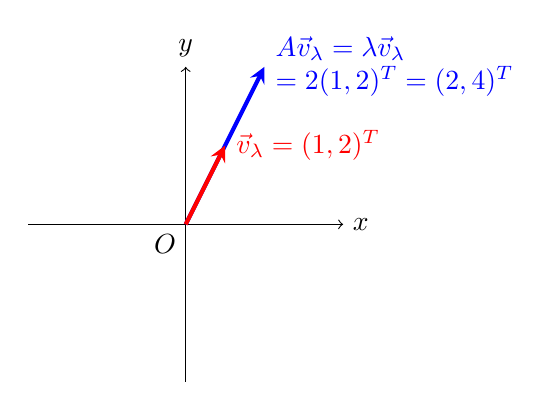
\begin{tikzpicture}
\draw[->] (-2,0)--(2,0) node[right]{$x$};
\draw[->] (0,-2)--(0,2) node[above]{$y$};
\draw[blue,-stealth,line width=1.5] (0,0)--(1,2) node[align=left, right]{$A\vec{v}_\lambda = \lambda\vec{v}_\lambda$\\ $= 2(1,2)^T = (2,4)^T$};
\draw[red,-stealth,line width=1.5] (0,0)--(1/2,1) node[anchor=west]{$\vec{v}_\lambda = (1,2)^T$};
\node[below left]{$O$}; 
\end{tikzpicture}
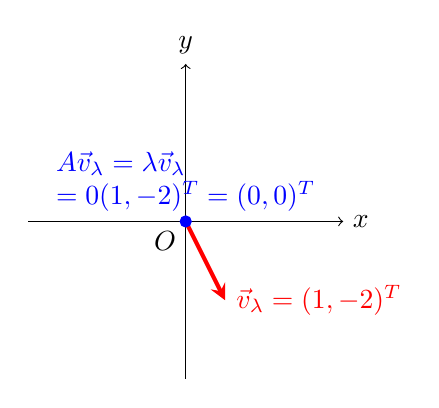
\begin{tikzpicture}
\draw[->] (-2,0)--(2,0) node[right]{$x$};
\draw[->] (0,-2)--(0,2) node[above]{$y$};
\draw[red,-stealth,line width=1.5] (0,0)--(1/2,-1) node[anchor=west]{$\vec{v}_\lambda = (1,-2)^T$};
\draw[blue, fill=blue] (0,0) circle[radius=2pt] node[align=left, above]{$A\vec{v}_\lambda = \lambda\vec{v}_\lambda$\\ $= 0(1,-2)^T = (0,0)^T$};
\node[below left]{$O$}; 
\end{tikzpicture}
\caption{\textit{Illustrations for the example above with $\lambda = 2 > 1$ (Extension), and $\lambda = 0$ (Vanished). The red/blue vector is before/after applying the linear transformation.}}
\end{figure}
There are infinitely many eigenvectors that are oriented in the same direction for a single eigenvalue, as seen in the remark of the last short exercise. Particularly, they are actually the span of any one of these (non-zero) eigenvectors. Thus, along a single direction, only one of them is needed for representation, and its span is at the same time a subspace by Properties \ref{proper:subspace_n_span}. This subspace is known as the \index{Eigenspace}\keywordhl{eigenspace} corresponding to that eigenvalue. Moreover, there may be more than one linearly independent eigenvector for the same eigenvalue, and the dimension of the eigenspace generated by them will be greater than one as well. In addition, the zero vector, technically, can be the eigenvector of any matrix since $A\vec{0} = \vec{0} = \lambda\vec{0}$ for any matrix $A$ and scalar $\lambda$. However, it is a trivial solution, plus more importantly, the zero vector is always linearly dependent by definition, and will not be taken into consideration (unlike the totally fine eigenvalue of zero).\par
Below is the visualization of some other possibilities for eigenvector rescaling.\footnotetext{
$
\begin{bmatrix}
1 & \frac{1}{2} \\
2 & 1
\end{bmatrix}
\left(s
\begin{bmatrix}
1 \\
2 
\end{bmatrix}\right)
=
s\begin{bmatrix}
1 & \frac{1}{2} \\
2 & 1
\end{bmatrix}
\begin{bmatrix}
1 \\
2 
\end{bmatrix}
=
s
\begin{bmatrix}
2 \\
4
\end{bmatrix}
=
2\left(s
\begin{bmatrix}
1 \\
2 
\end{bmatrix}\right)
$. In general, if $A\vec{v}_\lambda = \lambda\vec{v}_\lambda$ so that $\vec{v}_\lambda$ is some non-zero eigenvector, then $A(s\vec{v}_\lambda) = sA\vec{v}_\lambda = s\lambda\vec{v}_\lambda = \lambda(s\vec{v}_\lambda)$ and therefore all of its non-zero scalar multiples $s\vec{v}_\lambda$ are also an eigenvector.}
\begin{figure}[h!]
\centering
\begin{tikzpicture}
\draw[->] (-1.9,0)--(1.9,0) node[right]{$x$};
\draw[->] (0,-1.9)--(0,1.9) node[above]{$y$};
\draw[red,-stealth,line width=1.5] (0,0)--(-0.9,1.8);
\draw[blue,-stealth,line width=1.5] (0,0)--(-0.3,0.6);
\node[below left]{$O$}; 
\end{tikzpicture}
\begin{tikzpicture}
\draw[->] (-1.9,0)--(1.9,0) node[right]{$x$};
\draw[->] (0,-1.9)--(0,1.9) node[above]{$y$};
\draw[red,-stealth,line width=1.5] (0,0)--(1,0.5);
\draw[blue,-stealth,line width=1.5] (0,0)--(-0.8,-0.4);
\node[below left]{$O$}; 
\end{tikzpicture}
\begin{tikzpicture}
\draw[->] (-1.9,0)--(1.9,0) node[right]{$x$};
\draw[->] (0,-1.9)--(0,1.9) node[above]{$y$};
\draw[Green,-stealth,line width=1.5] (0,0)--(1.25,-0.65);
\node[below left]{$O$}; 
\end{tikzpicture}
\caption{\textit{Schematics of eigenvalues that represent: Contraction ($0 < \lambda < 1$), Reversal ($\lambda < 0$), Unchanged ($\lambda = 1$).}}
\end{figure}

\subsection{Finding Eigenvalues and Eigenvectors with Characteristic Polynomials}

To find the eigenvalues of a square matrix (or the linear transformation it represents), rearrange Equation (\ref{eqn:eigenmat}) in Definition \ref{defn:eigen} relating eigenvalues and eigenvectors to obtain
\begin{align}
A\vec{v}_\lambda &= \lambda\vec{v}_\lambda \nonumber \\
A\vec{v}_\lambda &= \lambda I\vec{v}_\lambda  &\text{($I\vec{v} = \vec{v}$ for any $\vec{v}$)} \nonumber  \\
(A-\lambda I)\vec{v}_\lambda &= \textbf{0} \label{eqn:eigenminus}
\end{align}
The last line constitutes a homogeneous linear system $B\vec{v}_\lambda = \vec{0}$ where $B = A - \lambda I$. For this system to have a non-trivial solution and hence an eigenvector, it is required that $\det(B) = \det(A - \lambda I) = 0$, as implied by Theorem \ref{thm:sqlinsysunique}. The relationship 
\begin{align}
p(\lambda) = \det(A - \lambda I) = 0    
\end{align}
is called the \index{Characteristic Equation/Polynomial}\keywordhl{characteristic equation}. The roots for $\lambda$ of the \textit{characteristic polynomial} $p(\lambda)$ are then the desired eigenvalues.
\begin{defn}[Characteristic Equation]
\label{defn:charactereqn}
The characteristic equation for a linear operator $T: \mathcal{V} \to \mathcal{V}$ over a vector space $\mathcal{V}$ with $\dim(\mathcal{V}) = n$ (or an $n \times n$ square matrix $A$) is
\begin{align*}
\det([T]_\beta - \lambda I) &= 0 & \text{ or } & & \det(A-\lambda I) = 0
\end{align*}
where $\mathcal{\beta}$ is any coordinate basis for $\mathcal{V}$. The L.H.S. ($p(\lambda) = \det([T]_B - \lambda I)$ or $\det(A-\lambda I)$), when expanded, constitutes a \keywordhl{characteristic polynomial} in $\lambda$ of degree $n$, the roots of which are the eigenvalues of $T$ (or $A$).
\end{defn}
$\blacktriangleright$ Short Exercise: By inspection, find all three eigenvalues of the matrix.\footnotemark
\begin{align*}
\begin{bmatrix}
1 & 0 & 0 \\
0 & 2 & 0 \\
0 & 0 & 3
\end{bmatrix}
\end{align*}
For each eigenvalue, there corresponds at least one linearly independent eigenvector by definition. The required eigenvector(s) that generates the eigenspace for a particular eigenvalue $\lambda_j$ can be found as the general solution to the matrix equation $(A - \lambda_j I)\vec{v} = \textbf{0}$ (see (\ref{eqn:eigenminus})), or in other words, (the basis for) the null space of $A - \lambda_j I$: $\mathcal{N}(A-\lambda_j I)$. The number of linearly independent eigenvectors (dimensions) in the eigenspace for $\lambda_j$ is hence the dimension of the null space (Definition \ref{defn:nullspace}) $\mathcal{N}(A-\lambda_j I)$, known as the \index{Geometric Multiplicity}\keywordhl{geometric multiplicity}. A closely related quantity is the \index{Algebraic Multiplicity}\keywordhl{algebraic multiplicity}, which is the number of times where $\lambda_j$ appears as the root to the characteristic polynomial. It can be shown that the geometric multiplicity of $\lambda_j$ is capped by its algebraic multiplicity.\footnotetext{They are $\lambda = 1,2,3$.}
\begin{thm}
\label{thm:geolessalgebra}
For an eigenvalue $\lambda_j$ to a square matrix $A$, its geometric multiplicity is equal to $\dim(\mathcal{N}(A-\lambda_j I))$, the dimension of the null space of $A-\lambda_j I$. Meanwhile, its algebraic multiplicity is the power $k_j$ of the factor $(\lambda_j - \lambda)^{k_j}$ present in the characteristic polynomial $p(\lambda)$. With these two quantities defined, we have
\begin{align*}
1 \leq \text{Geometric Multiplicity} \leq \text{Algebraic Multiplicity}
\end{align*}
for every distinct eigenvalue $\lambda_j$.
\end{thm}
We defer the proof showing that geometric multiplicity is always smaller than or equal to algebraic multiplicity until we introduce diagonalization later in this chapter.

\begin{exmp}
\label{exmp:dummyjordan}
Find all eigenvalues and eigenvectors for the matrix
\begin{align*}
A &=
\begin{bmatrix}
1 & -1 \\
0 & 1
\end{bmatrix}
\end{align*}
\end{exmp}
\begin{solution}
The characteristic equation is
\begin{align*}
p(\lambda) = \det(A - \lambda I) &= 
\begin{vmatrix}
1-\lambda & -1 \\
0 & 1-\lambda
\end{vmatrix} \\
&= (1-\lambda)^2 = 0
\end{align*}
Apparently, there is only one eigenvalue $\lambda = 1$, which has an algebraic multiplicity of $2$. Possible eigenvectors are then found by solving $A-\lambda I = \textbf{0}$:
\begin{align*}
\left[\begin{array}{@{}cc|c@{}}
1-1 & -1 & 0 \\
0 & 1-1 & 0
\end{array}\right] 
= 
\left[\begin{array}{@{}cc|c@{}}
0 & -1 & 0 \\
0 & 0 & 0
\end{array}\right]
\end{align*}
where the general solution is easily seen to be $t(1,0)^T$. So for the eigenvalue $\lambda = 1$, there is only one linearly independent eigenvector of $(1,0)^T$, which implies a geometric multiplicity of $1$.
\end{solution}

\begin{exmp}
\label{exmp:eigenfull}
For the matrix
\begin{align*}
A &= 
\begin{bmatrix}
1 & 3 & 1 \\
0 & 1 & 0 \\
1 & 0 & 2
\end{bmatrix}
\end{align*}
find its eigenvalues and eigenvectors.
\end{exmp}
\begin{solution}
The characteristic polynomial is, by Sarrus' Rule (Properties \ref{proper:sarrus})
\begin{align*}
\det(A-\lambda I) &= \begin{vmatrix}
1-\lambda & 3 & 1 \\
0 & 1-\lambda & 0 \\
1 & 0 & 2-\lambda 
\end{vmatrix} \\
&=
(1-\lambda)(1-\lambda)(2-\lambda) - (1)(1-\lambda)(1) \\
&= (1-\lambda)((2-3\lambda+\lambda^2) - 1) \\
&= (1-\lambda)(1-3\lambda+\lambda^2)
\end{align*}
The roots and thus eigenvalues are $\lambda = 1$ and
\begin{align*}
\lambda &= \frac{-(-3) \pm \sqrt{(-3)^2 - 4(1)(1)}}{2} \\
&= \frac{3}{2} \pm \frac{\sqrt{5}}{2}
\end{align*}
Particularly, for the eigenvalue $\lambda = \frac{3}{2} + \frac{\sqrt{5}}{2}$, the eigenvector is inferred from the homogeneous system $A - \lambda I = \textbf{0}$
\begin{align*}
& \left[\begin{array}{@{\,}wc{33pt}wc{30pt}wc{30pt}|c@{\,}}
-\frac{1}{2}-\frac{\sqrt{5}}{2} & 3 & 1 & 0 \\
0 & -\frac{1}{2}-\frac{\sqrt{5}}{2} & 0 & 0 \\
1 & 0 & \frac{1}{2}-\frac{\sqrt{5}}{2} & 0
\end{array}\right] \\
\to&
\left[\begin{array}{@{\,}wc{33pt}wc{30pt}wc{30pt}|c@{\,}}
1 & 0 & \frac{1}{2}-\frac{\sqrt{5}}{2} & 0 \\
0 & 1 & 0 & 0 \\
-\frac{1}{2}-\frac{\sqrt{5}}{2} & 3 & 1 & 0
\end{array}\right] & \begin{aligned}
R_1 &\leftrightarrow R_3 \\
\left(\frac{1}{-\frac{1}{2}-\frac{\sqrt{5}}{2}}\right)R_2 &\to R_2
\end{aligned} \\
\to&
\left[\begin{array}{@{\,}wc{33pt}wc{30pt}wc{30pt}|c@{\,}}
1 & 0 & \frac{1}{2}-\frac{\sqrt{5}}{2} & 0 \\
0 & 1 & 0 & 0 \\
0 & 3 & 0 & 0
\end{array}\right] & R_3 - \left(-\frac{1}{2}-\frac{\sqrt{5}}{2}\right)R_1 \to R_3 \\
\to&
\left[\begin{array}{@{\,}wc{33pt}wc{30pt}wc{30pt}|c@{\,}}
1 & 0 & \frac{1}{2}-\frac{\sqrt{5}}{2} & 0 \\
0 & 1 & 0 & 0 \\
0 & 0 & 0 & 0
\end{array}\right] & R_3 - 3R_2 \to R_3
\end{align*}
whose eigenvector can be seen to be $(-\frac{1}{2}+\frac{\sqrt{5}}{2},0,1)^T$ for $\lambda = \frac{3}{2} + \frac{\sqrt{5}}{2}$ by letting $z$ be the free variable.
\end{solution}
$\blacktriangleright$ Short Exercise: Find the eigenvectors for the other remaining eigenvalues.\footnotemark

\begin{exmp}
\label{exmp:2geomul}
Find all eigenvalues and eigenvectors for the matrix
\begin{align*}
A = \begin{bmatrix}
1 & 1 & -1 \\
-1 & 3 & -1 \\
1 & -1 & 3
\end{bmatrix}
\end{align*}
\end{exmp}
\begin{solution}
Again, the characteristic polynomial can be found by Sarrus' Rule as below.
\begin{align*}
p(\lambda) &= \det(A-\lambda I) \\
&= \begin{vmatrix}
1-\lambda & 1 & -1 \\
-1 & 3-\lambda & -1 \\
1 & -1 & 3-\lambda
\end{vmatrix} \\
&= [(1-\lambda)(3-\lambda)(3-\lambda) + (1)(-1)(1) + (-1)(-1)(-1)] \\
&\quad - [(-1)(3-\lambda)(1) + (1-\lambda)(-1)(-1) + (1)(-1)(3-\lambda)]\\
&= -\lambda^3 + 7\lambda^2 - 16\lambda + 12 \\
&= (2-\lambda)^2(3-\lambda)
\end{align*}
Hence the eigenvalues are $\lambda = 2,3$ with an algebraic multiplicity of $2$ and $1$ respectively. For $\lambda = 2$, its eigenvectors are retrieved via solving\footnotetext{For $\lambda = 1$, the eigenvector is $(-1,-\frac{1}{3},1)^T$. For $\lambda = \frac{3}{2} - \frac{\sqrt{5}}{2}$, it is $(-\frac{1}{2}-\frac{\sqrt{5}}{2},0,1)^T$. Note that for all three eigenvalues, their algebraic and geometric multiplicity are both $1$.}
\begin{align*}
\left[\begin{array}{@{\,}wc{17pt}wc{17pt}wc{17pt}|c@{\,}}
1-2 & 1 & -1 & 0 \\
-1 & 3-2 & -1 & 0 \\
1 & -1 & 3-2 & 0
\end{array}\right]
=& 
\left[\begin{array}{@{\,}wc{10pt}wc{10pt}wc{10pt}|c@{\,}}
-1 & 1 & -1 & 0 \\
-1 & 1 & -1 & 0 \\
1 & -1 & 1 & 0
\end{array}\right] \\ 
\to&
\left[\begin{array}{@{\,}wc{10pt}wc{10pt}wc{10pt}|c@{\,}}
1 & -1 & 1 & 0 \\
-1 & 1 & -1 & 0 \\
-1 & 1 & -1 & 0 
\end{array}\right] & R_1 \leftrightarrow R_3 \\
\to&
\left[\begin{array}{@{\,}wc{10pt}wc{10pt}wc{10pt}|c@{\,}}
1 & -1 & 1 & 0 \\
0 & 0 & 0 & 0 \\
0 & 0 & 0 & 0
\end{array}\right] & \begin{aligned}
R_2 + R_1 &\to R_2 \\
R_3 + R_1 &\to R_3 \\
\end{aligned}
\end{align*}
We have only one leading $1$ and two non-pivotal columns, so we can assign two free variables. For that, let $y = s$, $z = t$, then $x = s - t$. The general solution is then
\begin{align*}
\begin{bmatrix}
x \\
y \\ 
z
\end{bmatrix}
=
\begin{bmatrix}
s - t \\
s \\ 
t
\end{bmatrix}
=
s
\begin{bmatrix}
1 \\
1 \\
0
\end{bmatrix}
+ t 
\begin{bmatrix}
-1 \\
0 \\
1
\end{bmatrix}
\end{align*}
and hence the two linearly independent eigenvectors for $\lambda = 2$ are $(1,1,0)^T$ and $(-1,0,1)^T$. In this case, the geometric multiplicity is $2$ and is equal to the algebraic multiplicity. On the other hand, for $\lambda = 3$, we have
\begin{align*}
\left[\begin{array}{@{\,}wc{10pt}wc{10pt}wc{10pt}|c@{\,}}
-2 & 1 & -1 & 0 \\
-1 & 0 & -1 & 0 \\
1 & -1 & 0 & 0
\end{array}\right] 
&\to    
\left[\begin{array}{@{\,}wc{10pt}wc{10pt}wc{10pt}|c@{\,}}
1 & -1 & 0 & 0 \\
-1 & 0 & -1 & 0 \\
-2 & 1 & -1 & 0 
\end{array}\right] & R_1 \leftrightarrow R_3 \\
&\to    
\left[\begin{array}{@{\,}wc{10pt}wc{10pt}wc{10pt}|c@{\,}}
1 & -1 & 0 & 0 \\
0 & -1 & -1 & 0 \\
0 & -1 & -1 & 0 
\end{array}\right] & \begin{aligned}
R_2 + R_1 &\to R_2 \\
R_3 + 2R_1 &\to R_3
\end{aligned} \\
&\to    
\left[\begin{array}{@{\,}wc{10pt}wc{10pt}wc{10pt}|c@{\,}}
1 & -1 & 0 & 0 \\
0 & 1 & 1 & 0 \\
0 & -1 & -1 & 0 
\end{array}\right] & -R_2 \to R_2 \\
&\to    
\left[\begin{array}{@{\,}wc{10pt}wc{10pt}wc{10pt}|c@{\,}}
1 & -1 & 0 & 0 \\
0 & 1 & 1 & 0 \\
0 & 0 & 0 & 0 
\end{array}\right] & R_3 + R_2 \to R_3
\end{align*}
Now we have one non-pivotal column only and it is possible to take $z=t$ as the free variable. This will eventually yield $(-1,-1,1)^T$ as the only eigenvector for $\lambda = 3$.
\end{solution}

\begin{exmp}
\label{exmp:norealeig}
Show that 
\begin{align*}
A = \begin{bmatrix}
0 & -1 \\
1 & 0 
\end{bmatrix}
\end{align*}
admits no real eigenvalues. How about if we work over $\mathbb{C}$?
\end{exmp}
\begin{solution}
The characteristic equation is simply
\begin{align*}
p(\lambda) = \det(A-\lambda I) = \begin{vmatrix}
-\lambda & -1 \\
1 & -\lambda
\end{vmatrix} &= 0 \\
(-\lambda)^2 - (1)(-1) = \lambda^2 + 1 &= 0
\end{align*}
which has no real solution. So, if we are confined to work over $\mathbb{R}$ as the scalar for a real vector space, there is no possible eigenvalue $\lambda$ such that $A\vec{v}_\lambda = \lambda\vec{v}_\lambda$, as the scalar multiplication on R.H.S. only allows $\lambda$ to be a real number. Geometrically, for any (real) vector $\vec{v} = (x,y)^T$ on a flat plane, multiplying by $A$ leads to
\begin{align*}
A\vec{v} = 
\begin{bmatrix}
0 & -1 \\
1 & 0 
\end{bmatrix}
\begin{bmatrix}
x \\
y
\end{bmatrix}
=
\begin{bmatrix}
-y \\
x
\end{bmatrix}
\end{align*}
which rotates the vector in an anti-clockwise sense by $\SI{90}{\degree}$. So it is impossible for a vector to remain oriented in the same direction after $A$ is applied, consistent with the absence of any real eigenvalue. However, if we relax the constraint and work with $\mathbb{C}$, then the eigenvalues are clearly $\lambda = \pm i$. For $\lambda = i$, the eigenvector can be found from solving
\begin{align*}
\left[\begin{array}{@{\,}wc{10pt}wc{10pt}|c@{\,}}
-i & -1 & 0\\
1 &-i & 0
\end{array}\right]
\end{align*}
We can use a trick to immediately ignore the second row since the algebraic (and also geometric) multiplicity of $\lambda = i$ and hence the nullity of the system above is $1$, so there will be one redundant row, in this system which only has two rows. Now by considering the first row, we can easily find that the corresponding eigenvector is $(i,1)^T$. Similarly, the eigenvector of $\lambda = -i$ is $(-i,1)^T$. We will talk more about complex eigenvalues in Section \ref{subsection:diagcomplex} and Chapter \ref{chap:normalmat}.
\end{solution}

Some notable properties of eigenvalues and eigenvectors are provided below.
\begin{proper}
\label{proper:eigenlinind}
Eigenvectors for distinct eigenvalues are linearly independent.
\end{proper}
\begin{proof}
Let $\vec{v}^{(1)}$ and $\vec{v}^{(2)}$ be two eigenvectors corresponding to two different eigenvalues $\lambda_1$ and $\lambda_2$ of some square matrix $A$. By Theorem \ref{thm:linearindep}, we want to show that $c_1\vec{v}^{(1)} + c_2\vec{v}^{(2)} = \textbf{0}$ has the trivial solution $c_1 = c_2 = 0$ as the only solution. Now, applying $A$ to the left on both sides, we have
\begin{align*}
A(c_1\vec{v}^{(1)} + c_2\vec{v}^{(2)}) &= \textbf{0} \\
c_1(A\vec{v}^{(1)}) + c_2(A\vec{v}^{(2)}) &= \textbf{0} \\
c_1\lambda_1\vec{v}^{(1)} + c_2\lambda_2\vec{v}^{(2)} &= \textbf{0} & \text{(Definition \ref{defn:eigen})}
\end{align*}
But multiplying the same equation of $c_1\vec{v}^{(1)} + c_2\vec{v}^{(2)} = \textbf{0}$ by $\lambda_1$ gives $c_1\lambda_1\vec{v}^{(1)} + c_2\lambda_1\vec{v}^{(2)} = \textbf{0}$ instead. Subtracting this from the other equation leads to
\begin{align*}
(c_1\lambda_1\vec{v}^{(1)} + c_2\lambda_2\vec{v}^{(2)}) - (c_1\lambda_1\vec{v}^{(1)} + c_2\lambda_1\vec{v}^{(2)}) &= \textbf{0} - \textbf{0} \\
c_2(\lambda_2-\lambda_1)\vec{v}^{(2)} &= \textbf{0}
\end{align*}
Since $\lambda_1$ and $\lambda_2$ are distinct, $\lambda_2-\lambda_1 \neq 0$, and $\vec{v}^{(2)}$, being an eigenvector, cannot be the zero vector, the only possibility is $c_2 = 0$. The same argument shows that $c_1 = 0$, and we are done.
\end{proof}
\begin{proper}
\label{proper:eigentransinv}
For a square matrix $A$,
\begin{enumerate}
\item $A^T$ shares the same eigenvalues, but for each eigenvalue, the eigenvector(s) is/are not guaranteed to be the same. However, the dimensions (geometric multiplicity) of the two eigenspaces will be equal.
\item The eigenvalues for the inverse $A^{-1}$, provided that it exists, are the reciprocals of the eigenvalues of $A$, but the corresponding eigenvectors are the same.
\end{enumerate}
\end{proper}
\begin{proof}
For the first statement, note that
\begin{align*}
\det(A^T -\lambda I) &= \det(A^T - \lambda I^T) \\
&= \det((A - \lambda I)^T) & \text{(Properties \ref{proper:transp})} \\
&= \det(A - \lambda I) & \text{(Properties \ref{proper:properdet})}
\end{align*}
So the characteristic polynomials of $A$ and $A^T$ coincide, and the eigenvalues (if exist) will be the same. The geometric multiplicity can be shown to be equal by noting that transpose does not change the rank of a matrix, and thus $\text{rank}(A^T - \lambda I) = \text{rank}((A - \lambda I)^T) = \text{rank}(A - \lambda I)$. Subsequently, by using the Rank-nullity Theorem \ref{thm:ranknullity} twice, we have
\begin{align*}
\dim(\mathcal{N}(A^T-\lambda_j I)) &= n - \text{rank}(A^T - \lambda I) \\
&= n - \text{rank}(A - \lambda I) = \dim(\mathcal{N}(A-\lambda_j I))
\end{align*}
For the second statement, multiplying both sides of (\ref{eqn:eigenmat}) by $A^{-1}$ to obtain
\begin{align*}
A\vec{v}_\lambda &= \lambda\vec{v}_\lambda \\
A^{-1}A\vec{v}_\lambda = I\vec{v}_\lambda = \vec{v}_\lambda &= \lambda A^{-1}\vec{v}_\lambda & \text{(Definition \ref{defn:inverse})}\\
\frac{1}{\lambda}\vec{v}_\lambda &= A^{-1}\vec{v}_\lambda 
\end{align*}
which explicitly shows that $A^{-1}$ has $\frac{1}{\lambda}$ and $\vec{v}_\lambda$ as its eigenvalue and eigenvector.
\end{proof}
\begin{thm}
\label{thm:singularzeroeig}
A square matrix is singular if and only if it has zero as one of its eigenvalues.
\end{thm}
\begin{proof}
Exercise.\footnote{Denote the matrix by $A$, if it has an eigenvalue of zero, then by Definition \ref{defn:charactereqn}, $\det(A-0I) = 0 = \det(A)$. Properties \ref{proper:invnonzerodet} then imply $A$ is singular. The converse is established by the same argument in the reverse direction.} Note that this is also equivalent to $A$ having a non-trivial null space of dimension $\geq 1$ due to Theorem \ref{thm:geolessalgebra}.
\end{proof}

\subsection{Eigenspace as an Invariant Subspace}
The eigenspace actually belongs to a broader class of subspaces known as the \index{Invariant Subspaces}\keywordhl{invariant subspaces}. Given a linear operator $T: \mathcal{V} \to \mathcal{V}$, a subspace $\mathcal{W}$ of $\mathcal{V}$ is known as \textit{$T$-invariant} if applying $T$ to any vector $\vec{w} \in \mathcal{W}$ in the subspace maps it into a vector in the subspace $\mathcal{W}$ itself.
\begin{defn}[Invariant Subspace]
\label{defn:invariantsub}
With respect to a linear endomorphism $T: \mathcal{V} \to \mathcal{V}$, a $T$-invariant subspace $\mathcal{W} \subseteq \mathcal{V}$ is a subspace such that $T(\vec{w}) \in \mathcal{W}$ for all $\vec{w} \in \mathcal{W}$.
\end{defn}
The zero subspace and improper subspace ($\mathcal{V}$ itself) are two trivial invariant subspaces for any $T$. A more relevant fact is that any eigenspace of a fixed eigenvalue is $T$-invariant.
\begin{proper}
\label{proper:eigenTinvariant}
For a linear endomorphism $T: \mathcal{V} \to \mathcal{V}$, the eigenspace $\mathcal{E}_{J_i} \subseteq \mathcal{V}$ associated with a specific eigenvalue $\lambda_{J_i}$ is a $T$-invariant subspace.
\end{proper}
\begin{proof}
Exercise.\footnote{For any $\vec{w} \in \mathcal{E}_{J_i}$, by Definition \ref{defn:eigen}, $T(\vec{w}) = \lambda_{J_i} \vec{w} \in \mathcal{E}_{J_i}$. ((2) of Theorem \ref{thm:subspacecriteria})}
\end{proof}
and the same idea of an invariant subspace is applicable to any $n \times n$ square matrix $A$ and the real $n$-space $\mathbb{R}^n$. Another important observation is that for each of the linear transformations $T_{J_i}: \mathcal{W}_{J_i} \to \mathcal{W}_{J_i}$ (when they happen to be endomorphisms themselves) in their direct sum $T = \bigoplus_{J_i} T_{J_i}$ that is formed according to Definition \ref{defn:matdirectsum}, its corresponding subspace $\mathcal{W}_{J_i}$ (as in the vector direct sum $\mathcal{V} = \bigoplus_{J_i} \mathcal{W}_{J_i}$) is ($T_{J_i}$- and) $T$-invariant.

\subsection{Cayley-Hamilton Theorem}
We conclude this section by introducing the \index{Cayley-Hamilton Theorem}\keywordhl{Cayley-Hamilton Theorem}, which states that every square matrix satisfies its own characteristic equation, which means that replacing the $\lambda$ in the characteristic polynomial by the matrix results in a zero matrix.
\begin{thm}[Cayley-Hamilton Theorem]
\label{thm:CHthmmat}
For any $n \times n$ square matrix $A$, denote its characteristic polynomial by
\begin{align}
p(\lambda) = \det(A-\lambda I) = (-1)^n \sum_{k=0}^{n} c_k \lambda^k
\end{align}
where $c_n = 1$ is fixed, then we have
\begin{align}
p(A) = (-1)^n \sum_{k=0}^{n} c_k A^k = [\textbf{0}]
\end{align}
as an $n \times n$ zero matrix.
\end{thm}
One may be tempted to substitute $\lambda = A$ into $\det(A-\lambda I)$ to prove the Cayley-Hamilton Theorem. However, since $\lambda$ (and $\det(A-\lambda I)$) is a scalar but $A$ (and $[\textbf{0}]$) is a matrix, it is not a rigorous proof. A correct proof requires advanced knowledge, which is presented in Appendix \ref{section:B1}. Here, we will briefly see how it works.
\begin{exmp}
With the matrix
\begin{align*}
A = 
\begin{bmatrix}
1 & -1 \\
3 & 5
\end{bmatrix}
\end{align*}
verify the Cayley-Hamilton Theorem, and use the Cayley-Hamilton Theorem to evaluate $A^2 - 7A + 6I$.
\end{exmp}
\begin{solution}
The characteristic polynomial is
\begin{align*}
\begin{vmatrix}
1-\lambda & -1 \\
3 & 5-\lambda
\end{vmatrix}  
&= (1-\lambda)(5-\lambda) - (3)(-1) \\
&= 5 - 6 \lambda + \lambda^2 + 3 \\
&= \lambda^2 - 6\lambda + 8
\end{align*}
Replacing all $\lambda^k$ terms in the characteristic polynomial with $A^k$ (Notice that the constant term $c_0$ becomes $c_0 I$), we have
\begin{align*}
A^2 - 6A + 8I &= 
\begin{bmatrix}
1 & -1 \\
3 & 5
\end{bmatrix}^2
- 6
\begin{bmatrix}
1 & -1 \\
3 & 5
\end{bmatrix} 
+ 8
\begin{bmatrix}
1 & 0 \\
0 & 1
\end{bmatrix} \\
&=
\begin{bmatrix}
-2 & -6 \\
18 & 22
\end{bmatrix}
+
\begin{bmatrix}
-6 & 6 \\
-18 & -30
\end{bmatrix} 
+
\begin{bmatrix}
8 & 0 \\
0 & 8
\end{bmatrix} \\
&=
\begin{bmatrix}
0 & 0\\
0 & 0
\end{bmatrix}
\end{align*}
So the Cayley-Hamilton Theorem holds in this case. We can efficiently compute $A^2 - 7A + 6I$ through
\begin{align*}
A^2 - 7A + 6I &= (A^2 - 7A + 6I) - (A^2 - 6A + 8I) \\
&= -A-2I \\
&= -\begin{bmatrix}
1 & -1 \\
3 & 5
\end{bmatrix} 
-2
\begin{bmatrix}
1 & 0 \\
0 & 1
\end{bmatrix} \\
&=
\begin{bmatrix}
-3 & 1 \\
-3 & -7
\end{bmatrix}
\end{align*}
since $A^2 - 6A + 8I$ is a zero matrix.
\end{solution}

\section{Diagonalization}

\subsection{Mathematical Ideas of Diagonalization}
\label{section:diagonalizeidea}
The existence of eigenvectors allows us to carry out \index{Diagonalization}\keywordhl{diagonalization}, which helps us to simplify many linear algebra problems and derivations. A matrix $P$ is said to \textit{diagonalize} another matrix $A$ if the product $P^{-1}AP$ results in a \index{Diagonal Matrix}\keywordhl{diagonal matrix} $D$, where all non-zero entries are only found along the main diagonal.
\begin{defn}[Diagonalization]
A square matrix $A$ is diagonalizable, if there exists some \textit{invertible} square matrix $P$, such that
\begin{align}
P^{-1}AP = D
\end{align}
where $D$ is a diagonal matrix.
\end{defn}
Recalling Properties \ref{proper:endomorph}, we know that the form $P^{-1}AP$ (or $P^{-1}[T]P$ for a linear transformation) represents a change of coordinates for the matrix $A$. So the problem of diagonalization is actually asking if there exists a basis (expressed as the columns of $P$) such that the matrix $A$ in question is diagonal with respect to the corresponding coordinate system, or in other words, if $A$ is similar to a diagonal matrix. We will show that, in fact, the coordinate matrix $P$ required to diagonalize $A$, is formed by combining all linearly independent eigenvectors of $A$ column by column. This is only possible if the number of distinct eigenvectors is equal to the extent of $A$. An equivalent condition is that the characteristic polynomial splits over the scalar ($\mathbb{R}$ or $\mathbb{C}$)\footnotemark{} used in the vector space, and, for every eigenvalue, its geometric multiplicity is equal to the algebraic multiplicity.\footnotemark{} So, the matrix in Example \ref{exmp:dummyjordan} is non-diagonalizable. 
\begin{proper}
\label{proper:diagonalize}
An $n \times n$ square matrix $A$ can be diagonalized by another matrix $P$ if and only if $A$ has $n$ linearly independent eigenvectors, such that they form a basis for $\mathbb{R}^n$ (see part (b) of Properties \ref{proper:linindspanbasisnewver}) when the underlying scalar of vector space is taken to be $\mathbb{R}$ [a basis for $\mathbb{C}^n$ if working over $\mathbb{C}$]. The equivalent conditions are that the characteristic polynomial of $A$ splits over $\mathbb{R}$ [$\mathbb{C}$] and the geometric multiplicities of all distinct eigenvalues are equal to the respective algebraic multiplicities. Then, the columns of $P$ will consist of those eigenvectors $\smash{\vec{v}_\lambda^{(j)}}$, $j = 1,2,\ldots,n$. The diagonal entries of $P^{-1}AP = D$, are subsequently each of the eigenvalues $\lambda_j$ (counting repeated ones) corresponding to the eigenvector $\smash{\vec{v}_\lambda^{(j)}}$ in the same column position of $P$. 
\end{proper}
\footnotetext[\numexpr\value{footnote}-1]{\label{foot:split} A (characteristic) polynomial $p(\lambda)$ of degree $n$ is said to \index{Split}\textit{split} over $\mathbb{C}$ [$\mathbb{R}$] if it can be expressed as the product of linear factors only, i.e.\
\begin{align*}
p(\lambda) = \prod_{j=1}^n (\lambda_j - \lambda)    
\end{align*}
where $\lambda_j$ are complex [real] constants. Also, there is the \index{Fundamental Theorem of Algebra}\textit{Fundamental Theorem of Algebra} which states that every polynomial splits over $\mathbb{C}$ so the first part of the condition is automatically satisfied for the complex case.}\footnotetext{\label{foot:algequalgeo}Note that the sum of geometric multiplicities for all eigenvalues is less than or equal to (when the characteristic polynomial splits) the degree of the characteristic polynomial by observing Definition \ref{defn:charactereqn} and Theorem \ref{thm:geolessalgebra}, which is the same as the extent of the matrix. For the amount of linearly independent eigenvectors to be equal to that, the only possibility is that the geometric multiplicity of any eigenvalue is strictly equal to the algebraic multiplicity (Theorem \ref{thm:geolessalgebra} again) while $p(\lambda)$ splits. (Properties \ref{proper:eigenlinind} ensures linear independence over eigenspaces of different eigenvalues.)}
\begin{proof}
We will explicitly construct the desired form. Consider two matrix products $AP$ and $PD$, where $P = [\smash{\vec{v}_\lambda^{(1)}}|\smash{\vec{v}_\lambda^{(2)}}|\cdots|\smash{\vec{v}_\lambda^{(n)}}]$ contains the $n$ linearly independent eigenvectors as its columns. Then
\begin{align*}
AP &= A[\vec{v}_\lambda^{(1)}|\vec{v}_\lambda^{(2)}|\cdots|\vec{v}_\lambda^{(n)}] \\
&= [A\vec{v}_\lambda^{(1)}|A\vec{v}_\lambda^{(2)}|\cdots|A\vec{v}_\lambda^{(n)}] \\
&= [\lambda_1\vec{v}_\lambda^{(1)}|\lambda_2\vec{v}_\lambda^{(2)}|\cdots|\lambda_n \vec{v}_\lambda^{(n)}]
\end{align*}
where we have used Definition \ref{defn:eigen} and the first to second line can be referred to Footnote \ref{foot:factorleftmatrix} of Chapter \ref{chap:vec_space}. Also
\begin{align*}
PD &= [\vec{v}_\lambda^{(1)}|\vec{v}_\lambda^{(2)}|\cdots|\vec{v}_\lambda^{(n)}]
\begin{bmatrix}
\lambda_1 & 0 & \cdots & 0 \\
0 & \lambda_2 & & 0 \\
\vdots & & \ddots & \vdots \\
0 & 0 & \cdots & \lambda_n
\end{bmatrix} \\
&= [\lambda_1\vec{v}_\lambda^{(1)}|\lambda_2\vec{v}_\lambda^{(2)}|\cdots|\lambda_n \vec{v}_\lambda^{(n)}]
\end{align*}
So $AP = PD$. Notice that $P$ is invertible by (e) to (a) of Theorem \ref{thm:equiv3} since the columns of $P$ are made up of linearly independent eigenvectors by requirement, and thus $P^{-1}AP = D$.
\end{proof}

\subsection{Diagonalization for Real Eigenvalues}
\label{section:realeigen}

Before getting into the properties of diagonalization, let's see how diagonalization is carried out first. For a diagonalizable matrix with real eigenvalues, diagonalization is straightforward by the use of Properties \ref{proper:diagonalize}. Below is a worked example.
\begin{exmp}
Diagonalize the matrix 
\begin{align*}
A &= 
\begin{bmatrix}
1 & -2 & 1 \\ 
-\frac{2}{7} & 1 & -1 \\ 
-\frac{4}{7} & -2 & 0
\end{bmatrix}
\end{align*}
\end{exmp}
\begin{solution}
The characteristic polynomial can be checked to be 
\begin{align*}
p(\lambda) &= \det(A - \lambda I) \\
&= \begin{vmatrix}
1-\lambda & -2 & 1 \\ 
-\frac{2}{7} & 1-\lambda & -1 \\ 
-\frac{4}{7} & -2 & -\lambda
\end{vmatrix} \\
&= -\lambda^3 + 2\lambda^2 + \lambda - 2 = (-1-\lambda)(1-\lambda)(2-\lambda)
\end{align*}
Hence the eigenvalues are $\lambda = -1,1,2$. For $\lambda = -1$, the eigenvector is obtained from
\begin{align*}
\left[\begin{array}{@{\,}wc{36pt}wc{30pt}wc{30pt}|c@{\,}}
1-(-1) & -2 & 1 & 0\\ 
-\frac{2}{7} & 1-(-1) & -1 & 0\\ 
-\frac{4}{7} & -2 & -(-1) & 0
\end{array}\right] 
=& 
\left[\begin{array}{@{\,}wc{10pt}wc{10pt}wc{10pt}|c@{\,}}
2 & -2 & 1 & 0\\ 
-\frac{2}{7} & 2 & -1 & 0\\ 
-\frac{4}{7} & -2 & 1 & 0
\end{array}\right] \\
\to&
\left[\begin{array}{@{\,}wc{10pt}wc{10pt}wc{10pt}|c@{\,}}
1 & -1 & \frac{1}{2} & 0\\ 
-\frac{2}{7} & 2 & -1 & 0\\ 
-\frac{4}{7} & -2 & 1 & 0
\end{array}\right] & \frac{1}{2}R_1 \to R_1 \\
\to&
\left[\begin{array}{@{\,}wc{10pt}wc{10pt}wc{10pt}|c@{\,}}
1 & -1 & \frac{1}{2} & 0\\
0 & \frac{12}{7} & -\frac{6}{7} & 0\\
0 & -\frac{18}{7} & \frac{9}{7} & 0
\end{array}\right] &
\begin{aligned}
R_2 + \frac{2}{7}R_1 &\to R_2 \\
R_3 + \frac{4}{7}R_1 &\to R_3 \\
\end{aligned} \\
\to&
\left[\begin{array}{@{\,}wc{10pt}wc{10pt}wc{10pt}|c@{\,}}
1 & -1 & \frac{1}{2} & 0\\
0 & 1 & -\frac{1}{2} & 0\\
0 & -\frac{18}{7} & \frac{9}{7} & 0
\end{array}\right] & \frac{7}{12}R_2 \to R_2 \\
\to&
\left[\begin{array}{@{\,}wc{10pt}wc{10pt}wc{10pt}|c@{\,}}
1 & -1 & \frac{1}{2} & 0\\
0 & 1 & -\frac{1}{2} & 0\\
0 & 0 & 0 & 0
\end{array}\right] & R_3 + \frac{18}{7}R_2 \to R_3 \\
\to&
\left[\begin{array}{@{\,}wc{10pt}wc{10pt}wc{10pt}|c@{\,}}
1 & 0 & 0 & 0\\
0 & 1 & -\frac{1}{2} & 0\\
0 & 0 & 0 & 0
\end{array}\right] & R_1 + R_2 \to R_1
\end{align*}
The third column is non-pivotal and can be set as the free variable, which eventually leads to an eigenvector of $(0,1,2)^T$. We leave it to the readers to check that the eigenvectors for the remaining eigenvalues $\lambda = 1,2$ are $(-7,1,2)^T, (7,-3,1)^T$ respectively. Concatenating these three eigenvectors column by column yields
\begin{align*}
P &=
\begin{bmatrix}
0 & -7 & 7\\ 
1 & 1 & -3\\ 
2 & 2 & 1
\end{bmatrix}
\end{align*}
The diagonalization is then done according to Properties \ref{proper:diagonalize} as
\begin{align*}
D &= P^{-1}AP \\
&=
\begin{bmatrix}
0 & -7 & 7\\ 
1 & 1 & -3\\ 
2 & 2 & 1
\end{bmatrix}^{-1}
\begin{bmatrix}
1 & -2 & 1 \\ 
-\frac{2}{7} & 1 & -1 \\ 
-\frac{4}{7} & -2 & 0
\end{bmatrix}
\begin{bmatrix}
0 & -7 & 7\\ 
1 & 1 & -3\\ 
2 & 2 & 1
\end{bmatrix} \\
&=
\begin{bmatrix}
\frac{1}{7}&\frac{3}{7}&\frac{2}{7}\\ 
-\frac{1}{7}&-\frac{2}{7}&\frac{1}{7}\\ 
0&-\frac{2}{7}&\frac{1}{7}
\end{bmatrix}
\begin{bmatrix}
0&-7&14\\ 
-1&1&-6\\ 
-2&2&2
\end{bmatrix} \\
&=
\begin{bmatrix}
-1 & 0 & 0 \\
0 & 1 & 0 \\
0 & 0 & 2
\end{bmatrix}
\end{align*}
Note that we can shuffle the ordering of the eigenvalues and eigenvectors.\footnote{For example, \begin{align*}
\begin{bmatrix}
0 & 7 & -7 \\ 
1 & -3 & 1 \\ 
2 & 1 & 2 
\end{bmatrix}^{-1}
\begin{bmatrix}
1 & -2 & 1 \\ 
-\frac{2}{7} & 1 & -1 \\ 
-\frac{4}{7} & -2 & 0
\end{bmatrix}
\begin{bmatrix}
0 & 7 & -7 \\ 
1 & -3 & 1 \\ 
2 & 1 & 2 
\end{bmatrix} 
=
\begin{bmatrix}
-1 & 0 & 0 \\
0 & 2 & 0 \\
0 & 0 & 1
\end{bmatrix}
\end{align*} is another valid outcome where we have interchanged the second and third eigenvector.} We therefore say that diagonalization is \textit{unique up to a permutation}.
\end{solution}
$\blacktriangleright$ Short Exercise: Reverse the diagonalization to recover the original matrix.\footnotemark

\begin{exmp}
Diagonalize the matrix 
\begin{align*}
A = \begin{bmatrix}
1 & 1 & -1 \\
-1 & 3 & -1 \\
1 & -1 & 3
\end{bmatrix}
\end{align*}
in Example \ref{exmp:2geomul}.
\end{exmp}
\begin{solution}
From Example \ref{exmp:2geomul}, we know that the characteristic polynomial splits over $\mathbb{R}$, and for the eigenvalues of $\lambda = 2,3$, their geometric multiplicities are equal to algebraic multiplicities ($2$ and $1$). Therefore, its diagonalization is possible by Properties \ref{proper:diagonalize}. Specifically, the eigenvectors for $\lambda = 2$ are $(1,1,0)^T, (-1,0,1)^T$ and that for $\lambda = 3$ is $(-1,-1,1)^T$. Thus we have
\begin{align*}
P &= 
\begin{bmatrix}
1 & -1 & -1 \\
1 & 0 & -1 \\
0 & 1 & 1
\end{bmatrix}
\text{ and} \\
D &= P^{-1}AP \\
&= \begin{bmatrix}
1 & -1 & -1 \\
1 & 0 & -1 \\
0 & 1 & 1
\end{bmatrix}^{-1}
\begin{bmatrix}
1 & 1 & -1 \\
-1 & 3 & -1 \\
1 & -1 & 3
\end{bmatrix}
 \begin{bmatrix}
1 & -1 & -1 \\
1 & 0 & -1 \\
0 & 1 & 1
\end{bmatrix} \\
&= 
\begin{bmatrix}
1 & 0 & 1 \\
-1 & 1 & 0 \\
1 & -1 & 1
\end{bmatrix}
\begin{bmatrix}
2 & -2 & -3 \\
2 & 0 & -3 \\
0 & 2 & 3
\end{bmatrix} \\
&= 
\begin{bmatrix}
2 & 0 & 0 \\
0 & 2 & 0 \\
0 & 0 & 3
\end{bmatrix}
\end{align*}
The first and second eigenvectors can be interchanged without modifying the form of the diagonalized matrix as they correspond to the same eigenvalue of $\lambda = 2$.
\end{solution}
\footnotetext{Simply compute $PDP^{-1}$ which should be equal to $A$.}

\subsection{Properties of Diagonalization}
\label{section:diagonalproper}

Having seen the actual procedure of diagonalization, we are ready to derive its properties. First, it is instructive to view diagonalization from the perspective of a vector/matrix direct sum. The condition in Properties \ref{proper:diagonalize} requires that there are $n$ one-dimensional subspaces $\mathcal{E}_j$ generated by each of the $n$ linearly independent eigenvectors $\smash{\vec{v}_\lambda^{(j)}}$ for the linear operator $T: \mathcal{V} \to \mathcal{V}$ (can be treated as an $n \times n$ square matrix $A$) where $\mathcal{V}$ is an $n$-dimensional vector space, and thus they form a direct sum $\bigoplus_{j=1}^n \mathcal{E}_j = \mathcal{V}$ (or $\mathbb{R}^n$/$\mathbb{C}^n$) following Definition \ref{defn:directsum} and Properties \ref{proper:linindspanbasisnewver}. In Properties \ref{proper:eigenTinvariant}, we have already observed that the eigenspace $\mathcal{E}_{J_i} = \bigoplus_{\lambda_j = \lambda_{J_i}} \mathcal{E}_j$ of each distinct eigenvalue $\lambda_{J_i}$\footnote{$J_i$ refers to the set of indices those are associated to a common eigenvalue, denoted by $\lambda_{J_i}$.} is an invariant subspace under $T$ and the same can be said for the individual one-dimensional $\mathcal{E}_j$ themselves. In particular, the direction of any vector in each of the eigenspaces remains unchanged after $T$ is applied. Therefore, by Definition \ref{defn:matdirectsum}, $T$ can be written as a matrix direct sum $T = \bigoplus_{j=1}^n T_j$ where $T_j(\smash{\vec{v}_\lambda^{(j)}}): \mathcal{E}_j \to \mathcal{E}_j = T|_{\mathcal{E}_j}(\smash{\vec{v}_\lambda^{(j)}}) = T(\smash{\vec{v}_\lambda^{(j)}}) = \lambda_j\smash{\vec{v}_\lambda^{(j)}} = \lambda_j(\text{id}(\smash{\vec{v}_\lambda^{(j)}}))$. In matrix representation, it becomes $A = \bigoplus_{j=1}^n [\lambda_j]$ where each of the $[\lambda_j]$ is a singleton ($1 \times 1$) block. If we consider repeated eigenvalues and their full eigenspaces $\smash{\mathcal{E}_{J_i} = \bigoplus_{\lambda_j = \lambda_{J_i}} \mathcal{E}_j}$ as an entirety, then we have $\smash{T = \bigoplus_{\text{all distinct }\lambda_{J_i}} T_{J_i}}$ with simply $T_{J_i} = \lambda_{J_i}(\text{id}[\,]): \mathcal{E}_{J_i} \to \mathcal{E}_{J_i}$ and the matrix form is $\smash{A = \bigoplus_{\text{all distinct }\lambda_{J_i}} \lambda_{J_i} I_{k_{J_i}}}$ where $k_{J_i}$ is the eigenvalue repetition count of $\lambda_{J_i}$ in the characteristic polynomial (here the algebraic multiplicity is equal to the geometric counterpart as required by Properties \ref{proper:diagonalize}). The essence of diagonalization is hence to find a basis for $\mathcal{V}$ as a vector direct sum such that $T: \mathcal{V} \to \mathcal{V}$ becomes a matrix direct sum that is composed by some scalar multiples of identity matrices/identity mappings with respect to this vector direct sum basis.

On the other hand, the original matrix $A$ and its diagonalized form $D = P^{-1}AP$ share some similarities sometimes called \index{Invariant (Matrix)}\keywordhl{invariants}. More generally, these invariants hold for any pair of similar matrices (introduced following Properties \ref{proper:endomorph}). 
\begin{proper}[Invariants for Similar Matrices]
\label{proper:similarinvariant}
Two similar square matrices $A$ and $A'$ have the
\begin{enumerate}
\item same determinant;
\item same characteristic equation;
\item same eigenvalues and algebraic multiplicities;
\item same eigenspace dimension (geometric multiplicity) for any fixed eigenvalue (but the eigenvectors are probably different);
\item same trace, a.k.a.\ the sum of diagonal entries; and
\item same rank.
\end{enumerate}
\end{proper}
\begin{proof}
We will briefly prove (1) here. Similar matrices are related by $A' = P^{-1}AP$ for any invertible matrix $P$. As a result, $\det(A') = \det(P^{-1}AP) = \det(P^{-1})\det(A)\det(P) = \frac{1}{\det(P)}\det(A)\det(P) = \det(A)$ due to Properties \ref{proper:properdet}. ($\det(P) \neq 0$ by Properties \ref{proper:invnonzerodet}.)
\end{proof}
Since the diagonalized form of a matrix is clearly similar to the original one, those properties hold for them as well.\par
$\blacktriangleright$ Short Exercise: Prove (2) and (3) of the above properties.\footnotemark\par

With all of these, we can finally prove Theorem \ref{thm:geolessalgebra} now. Denote the geometric multiplicity of $A$ by $n_{J_i}$ for a fixed eigenvalue $\lambda_{J_i}$. Then the $n_{J_i}$ linearly independent eigenvectors $\smash{\vec{v}_{\lambda_{J_i}}^{(1)}, \vec{v}_{\lambda_{J_i}}^{(2)}, \ldots, \vec{v}_{\lambda_{J_i}}^{(n_{J_i})}}$ accordingly will lead to an $n_{J_i}$-dimensional eigenspace of $\mathcal{E}_{J_i} = \smash{\bigoplus_{\lambda_j = \lambda_{J_i}} \mathcal{E}_j}$ as just described, that is, an invariant subspace under the multiplication by $A$ to its left. We can always enlarge (the basis of) this eigenspace $\mathcal{E}_{J_i}$ to reproduce the entire $\mathbb{R}^n$ (or $\mathbb{C}^n$) as suggested by part (c) of Properties \ref{proper:linindspanbasisnewver}. If we do a change of coordinates on $A$ using this new basis, then it will become (Properties \ref{proper:endomorph} again)
\begin{align*}
A' = P^{-1}AP
\end{align*}
where
\begin{align*}
P = \begin{bmatrix}
\vec{v}_{\lambda_{J_i}}^{(1)}|\vec{v}_{\lambda_{J_i}}^{(2)}|\ldots|\vec{v}_{\lambda_{J_i}}^{(n_{J_i})}|\text{other vectors used to fill the basis for $\mathbb{R}^n$}
\end{bmatrix}
\end{align*}
Compared with our discussion just before and according to Definition \ref{defn:matrixrepoflintrans}, we know that the new matrix $A'$ will take the block form of
\begin{align*}
A' = 
\begin{bmatrix}
\lambda_{J_i} I_{n_{J_i}} & *_{n_{J_i}\times(n-n_{J_i})} \\
[\textbf{0}]_{(n-n_{J_i})\times n_{J_i}} & *_{(n-n_{J_i})\times(n-n_{J_i})}
\end{bmatrix}
\end{align*}
\footnotetext{$\det(A'-\lambda I) = \det(P^{-1}AP-\lambda I) = \det(P^{-1}AP-\lambda P^{-1}P) = \det(P^{-1}AP-\lambda P^{-1}IP) = \det(P^{-1}(A-\lambda I)P) = \det(P^{-1})\det(A-\lambda I)\det(P) = \det(A-\lambda I)$ (Definition \ref{defn:inverse}, Properties \ref{proper:identity} and \ref{proper:properdet}). (3) follows from (2) immediately.}\footnote{We can check if the first $n_j$ columns are equal for $PA'$ and $AP$, which is very similar to the derivation in Properties \ref{proper:diagonalize}.
\begin{align*}
PA' &= \begin{bmatrix}
\vec{v}_{\lambda_{J_i}}^{(1)}|\vec{v}_{\lambda_{J_i}}^{(2)}|\ldots|\vec{v}_{\lambda_{J_i}}^{(n_{J_i})}|*
\end{bmatrix}
\begin{bmatrix}
\lambda_{J_i} I_{n_{J_i}} & *_{n_{J_i}\times(n-n_{J_i})} \\
[\textbf{0}]_{(n-n_{J_i})\times n_{J_i}} & *_{(n-n_{J_i})\times(n-n_{J_i})}
\end{bmatrix} \\
&=
\begin{bmatrix}
\lambda_{J_i}\vec{v}_{\lambda_{J_i}}^{(1)}|\lambda_{J_i}\vec{v}_{\lambda_{J_i}}^{(2)}|\ldots|\lambda_{J_i}\vec{v}_{\lambda_{J_i}}^{(n_{J_i})}|*
\end{bmatrix}
\end{align*} and
\begin{align*}
AP &= A\begin{bmatrix}
\vec{v}_{\lambda_{J_i}}^{(1)}|\vec{v}_{\lambda_{J_i}}^{(2)}|\ldots|\vec{v}_{\lambda_{J_i}}^{(n_{J_i})}|*
\end{bmatrix} \\
&= 
\begin{bmatrix}
A\vec{v}_{\lambda_{J_i}}^{(1)}|A\vec{v}_{\lambda_{J_i}}^{(2)}|\ldots|A\vec{v}_{\lambda_{J_i}}^{(n_{J_i})}|*
\end{bmatrix} \\
&= \begin{bmatrix}
\lambda_{J_i}\vec{v}_{\lambda_{J_i}}^{(1)}|\lambda_{J_i}\vec{v}_{\lambda_{J_i}}^{(2)}|\ldots|\lambda_{J_i}\vec{v}_{\lambda_{J_i}}^{(n_{J_i})}|*
\end{bmatrix}
\end{align*}
the last step is by the definition of eigenvectors (Definition \ref{defn:eigen}).} where the top left block represents a rescaling of the eigenvectors (now as a part of the new basis) by the eigenvalue, and the $*$ parts can be anything (notice the zero block at the bottom left, since $\mathcal{E}_{J_i}$ is an invariant subspace). Its characteristic polynomial is then 
\begin{align*}
\det(A'-\lambda I) =
\begin{vmatrix}
(\lambda_{J_i}-\lambda) I_{n_{J_i}} & *_{n_{J_i}\times(n-n_{J_i})} \\
[\textbf{0}]_{(n-n_{J_i})\times n_{J_i}} & *_{(n-n_{J_i})\times(n-n_{J_i})}-\lambda I_{(n-n_{J_i})}    
\end{vmatrix}
\end{align*}
By repeated cofactor expansion along the first $n_{J_i}$ columns, we have
\begin{align*}
p(\lambda) = (\lambda_{J_i}-\lambda)^{n_{J_i}} \det(*_{(n-n_{J_i})\times(n-n_{J_i})}-\lambda I_{(n-n_{J_i})})
\end{align*}
which shows that the characteristic polynomial has $\lambda_{J_i}$ as its roots occurring for at least $n_{J_i}$ times (the determinant that follows may or may not have any $(\lambda_{J_i}-\lambda)$ factor). By Properties \ref{proper:similarinvariant}, the original matrix $A$ will share the same characteristic polynomial and hence the algebraic multiplicity for $\lambda_{J_i}$ (the times where the $(\lambda_{J_i}-\lambda)$ factor appears in the characteristic polynomial) concerning $A$ will be greater than or equal to its given geometric multiplicity $n_{J_i}$.\par

Diagonalization also enables the efficient computation of matrix powers, as demonstrated in the following example.

\begin{exmp}
\label{exmp:powerdiag}
Show that for
\begin{align*}
A = 
\begin{bmatrix}
\frac{3}{2} & \frac{1}{2} \\
\frac{1}{2} & \frac{3}{2}
\end{bmatrix}
\end{align*}
its successive power is
\begin{align*}
A^n =
\begin{bmatrix}
\frac{1}{2}(2^n + 1) & \frac{1}{2}(2^n - 1) \\
\frac{1}{2}(2^n - 1) & \frac{1}{2}(2^n + 1)
\end{bmatrix}
\end{align*}
\end{exmp}
\begin{solution}
We leave it to the readers to show that the diagonalization of $A$ is done by
\begin{align*}
D &= P^{-1}AP \\
\begin{bmatrix}
2 & 0 \\
0 & 1
\end{bmatrix} &=
\begin{bmatrix}
1 & -1 \\
1 & 1
\end{bmatrix}^{-1}
\begin{bmatrix}
\frac{3}{2} & \frac{1}{2} \\
\frac{1}{2} & \frac{3}{2}
\end{bmatrix} 
\begin{bmatrix}
1 & -1 \\
1 & 1
\end{bmatrix}
\end{align*}
Hence
\begin{align*}
A^n &= (PDP^{-1})^n \\
&= (PDP^{-1})(PDP^{-1})\cdots(PDP^{-1})(PDP^{-1}) \\
&= PD(P^{-1}P)D\cdots D(P^{-1}P)P^{-1} \\
&= PDID \cdots DIP^{-1} & \text{(Definition \ref{defn:inverse})} \\
&= PD^nP^{-1} \\
&= \begin{bmatrix}
1 & -1 \\
1 & 1
\end{bmatrix}
\begin{bmatrix}
2^n & 0 \\
0 & 1^n
\end{bmatrix}
\begin{bmatrix}
1 & -1 \\
1 & 1
\end{bmatrix}^{-1} \\
&= 
\begin{bmatrix}
1 & -1 \\
1 & 1
\end{bmatrix}
\begin{bmatrix}
2^n & 0 \\
0 & 1
\end{bmatrix}
\begin{bmatrix}
\frac{1}{2} & \frac{1}{2} \\
-\frac{1}{2} & \frac{1}{2} 
\end{bmatrix} \\
&= \begin{bmatrix}
\frac{1}{2}(2^n + 1) & \frac{1}{2}(2^n - 1) \\
\frac{1}{2}(2^n - 1) & \frac{1}{2}(2^n + 1)
\end{bmatrix}
\end{align*}
where the successive powers of a diagonal matrix can be simply computed over each of the diagonal entries.
\end{solution}

\subsection{Diagonalization for Complex Eigenvalues}
\label{subsection:diagcomplex}
It is not uncommon for a real square matrix $A$ to have complex eigenvalues (as well as complex eigenvectors). In such cases, to perform diagonalization, one possible approach is following exactly what we have done in Section \ref{section:realeigen} to produce $D = P^{-1}AP$ which contains the complex eigenvalues along its main diagonal (and are all zeros elsewhere) if we choose to work over $\mathbb{C}$. This can be useful sometimes, but the downside is that $D$ (as well as the $P$ matrix that is made up of the eigenvectors as its columns) is comprised of complex entries, despite $A$ being a real matrix. There is, indeed, another method that uses the property of complex numbers introduced in the last chapter, which circumvents the appearance of complex numbers in a modified diagonalized form and allows us to stay in the world of $\mathbb{R}$. But first of all, we need to introduce a basic theorem about the complex roots of an equation.
\begin{thm}
For a \textit{real} polynomial equation of order $n$
\begin{align*}
p(x) = \sum_{k=0}^{n} c_k x^k
\end{align*}
such that the coefficients $c_k$ are all real numbers. If $z_0 = a+bi$ is a complex root so that $p(z_0) = \sum_{k=0}^{n} c_k z_0^k = 0$, where $a$ and $b$ are real constants, then its conjugate $\overline{z_0} = a-bi$ is also another root for the equation.
\end{thm}
\begin{proof}
By Properties \ref{proper:complexnum}, if we take the complex conjugate on both sides of the real polynomial equation with $x = z_0$, then
\begin{align*}
\overline{p(z_0)} &= \overline{\sum_{k=0}^{n} c_k z_0^k} = \overline{0} \\
&= \sum_{k=0}^{n} \overline{c_k} \overline{z_0^k} = 0 \\
{p(\overline{z_0})} &= \sum_{k=0}^{n} c_k \overline{z_0}^k = 0
\end{align*}
$\overline{c_k} = c_k$ as they are real coefficients.
\end{proof}
Since the characteristic polynomial must be a real polynomial for a real matrix $A$, by the theorem we have just proved, we know that its complex roots and hence the complex eigenvalues of $A$ always come in a conjugate pair. For a pair of complex eigenvalues, their eigenvectors are also the conjugate of each other.
\begin{proper}
\label{proper:eigenconj}
If $\lambda_0$ is a complex eigenvalue for a real matrix $A$ with an eigenvector of $\vec{v}_{\lambda_0}$, then $A$ also has $\overline{\lambda_0}$ and $\overline{\vec{v}_{\lambda_0}}$ as another eigenvalue and eigenvector.
\end{proper}
\begin{proof}
By Definition \ref{defn:eigen},
\begin{align*}
A\vec{v}_{\lambda_0} &= \lambda_0\vec{v}_{\lambda_0}    
\end{align*}
Taking complex conjugate on both sides, we have
\begin{align*}
\overline{A\vec{v}_{\lambda_0}} &= \overline{\lambda_0\vec{v}_{\lambda_0}} \\
A \overline{\vec{v}_{\lambda_0}} &= \overline{\lambda_0}\, \overline{\vec{v}_{\lambda_0}}
\end{align*}
with the use of Properties \ref{proper:complexnum}, and noting that $\overline{A} = A$ as $A$ is a real matrix.
\end{proof}
Now as we know that complex eigenvalues and eigenvectors always appear as a pair of conjugates, and conjugates share the same real and imaginary parts except a sign difference for the latter, we are encouraged to use them like two different eigenvalues and eigenvectors for making up. The following properties show that it is possible to take advantage of this and derive a new diagonalization procedure with some tweaks.

\begin{proper}
\label{proper:diagonalize2}
For a real square matrix $A$, the procedure in Properties \ref{proper:diagonalize} can be adapted for a complex eigenvalue $\lambda_0 = \Re{\lambda_0} + i \Im{\lambda_0}$, the corresponding eigenvector $\vec{v}_{\lambda_0} = \Re{\vec{v}_{\lambda_0}} + i \Im{\vec{v}_{\lambda_0}}$, as well as their complex conjugates, by replacing the corresponding columns in
\begin{align*}
&P = [\cdots|\vec{v_{\lambda_0}}|\overline{\vec{v_{\lambda_0}}}|\cdots]
&D =
\begin{bmatrix}
\ddots & 0 & 0 & \\
& \lambda_0 & 0 & \\
& 0 & \overline{\lambda_0} & \\
& 0 & 0 & \ddots
\end{bmatrix}
\end{align*}
by
\begin{align}
&P = [\cdots|\Re{\vec{v}_{\lambda_0}}|\Im{\vec{v}_{\lambda_0}}|\cdots]
&D =
\begin{bmatrix}
\ddots & 0 & 0 & \\
& \Re{\lambda_0} & \Im{\lambda_0} & \\
& -\Im{\lambda_0} & \Re{\lambda_0} & \\
& 0 & 0 & \ddots
\end{bmatrix}
\label{eqn:diagonalize2}
\end{align}
\end{proper}
\begin{proof}
As in the proof for Properties \ref{proper:diagonalize}, we set out to prove that $AP = PD$ for the two columns concerned. To make it easier to read, denote $\Re{\lambda_0} = a$ and $\Im{\lambda_0} = b$. It is not hard to see that
\begin{align*}
PD &=
[\cdots|\Re{\vec{v}_{\lambda_0}}|\Im{\vec{v}_{\lambda_0}}|\cdots]
\begin{bmatrix}
\ddots & 0 & 0 & \\
& a & b & \\
& -b & a & \\
& 0 & 0 & \ddots
\end{bmatrix} \\
&= [\cdots|a\Re{\vec{v}_{\lambda_0}} - b\Im{\vec{v}_{\lambda_0}} | b\Re{\lambda_0} + a\Im{\vec{v}_{\lambda_0}}|\cdots]
\end{align*}
(Properties \ref{proper:linearcombmatrix}) On the other hand, notice that the relation between the complex eigenvalue and eigenvector via Definition \ref{defn:eigen} can be expanded as
\begin{align*}
A\vec{v}_{\lambda_0} &= \lambda_0\vec{v}_{\lambda_0} \\
A(\Re{\vec{v}_{\lambda_0}} + i \Im{\vec{v}_{\lambda_0}}) &= (a+bi)(\Re{\vec{v}_{\lambda_0}} + i \Im{\vec{v}_{\lambda_0}}) \\
A\Re{\vec{v}_{\lambda_0}} + i A\Im{\vec{v}_{\lambda_0}} &= \begin{aligned}
& (a\Re{\vec{v}_{\lambda_0}} - b\Im{\vec{v}_{\lambda_0}}) \\
& +i(b\Re{\vec{v}_{\lambda_0}} + a\Im{\vec{v}_{\lambda_0}})    
\end{aligned}
\end{align*}
where $\Re{\vec{v}_{\lambda_0}}$ and $\Im{\vec{v}_{\lambda_0}}$ themselves are real vectors and $A$ is a real matrix. By equating the real and imaginary parts, we have
\begin{subequations}
\begin{align}
A\Re{\vec{v}_{\lambda_0}} &= a\Re{\vec{v}_{\lambda_0}} - b\Im{\vec{v}_{\lambda_0}} \label{eqn:realmodiag} \\
A\Im{\vec{v}_{\lambda_0}} &= b\Re{\vec{v}_{\lambda_0}} + a\Im{\vec{v}_{\lambda_0}}
\label{eqn:imgmodiag}
\end{align}
\end{subequations}
Hence
\begin{align*}
AP &= A[\cdots|\Re{\vec{v}_{\lambda_0}}|\Im{\vec{v}_{\lambda_0}}|\cdots] \\
&= [\cdots|A\Re{\vec{v}_{\lambda_0}}|A\Im{\vec{v}_{\lambda_0}}|\cdots] \\
&= [\cdots|a\Re{\vec{v}_{\lambda_0}} - b\Im{\vec{v}_{\lambda_0}} | b\Re{\lambda_0} + a\Im{\vec{v}_{\lambda_0}}|\cdots] \\
&= PD
\end{align*}
The only caveat is to prove that $P$ is invertible, or equivalently $\Re{\vec{v}_{\lambda_0}}$ and $\Im{\vec{v}_{\lambda_0}}$ are linearly independent (assuming there is no problem with other columns). We can prove that by assuming they are linearly dependent, so $\Re{\vec{v}_{\lambda_0}} = k\Im{\vec{v}_{\lambda_0}}$ for some \textit{real} constant $k$, and plugging this into the expressions of $A\Re{\vec{v}_{\lambda_0}}$ and $A\Im{\vec{v}_{\lambda_0}}$ to derive a contradiction.\footnote{Substitute $\Re{\vec{v}_{\lambda_0}} = k\Im{\vec{v}_{\lambda_0}}$ into Equation (\ref{eqn:realmodiag})
\begin{align*}
A\Re{\vec{v}_{\lambda_0}} &= a\Re{\vec{v}_{\lambda_0}} - b\Im{\vec{v}_{\lambda_0}} \\
Ak\Im{\vec{v}_{\lambda_0}} &= ak\Im{\vec{v}_{\lambda_0}} - b\Im{\vec{v}_{\lambda_0}} = (ak-b)\Im{\vec{v}_{\lambda_0}}
\end{align*}
and multiplying Equation (\ref{eqn:imgmodiag}) by $k$
\begin{align*}
A\Im{\vec{v}_{\lambda_0}} &= b\Re{\vec{v}_{\lambda_0}} + a\Im{\vec{v}_{\lambda_0}} \\
Ak \Im{\vec{v}_{\lambda_0}} &= bk(k\Im{\vec{v}_{\lambda_0}}) + ak\Im{\vec{v}_{\lambda_0}} = (bk^2 + ak)\Im{\vec{v}_{\lambda_0}}
\end{align*}
Comparing these two equations ($\Re{\vec{v}_{\lambda_0}}$ and $\Im{\vec{v}_{\lambda_0}}$ are \text{non-zero, real} vectors) gives
\begin{align*}
bk^2 + ak = ak - b \implies bk^2 = -b \implies k = \pm i
\end{align*}
which contradicts the assumption where $k$ has to be real.}
\end{proof}

The block in the form
\begin{align*}
\begin{bmatrix}
\ddots & 0 & 0 & \\
& a & b & \\
& -b & a & \\
& 0 & 0 & \ddots
\end{bmatrix}    
\end{align*}
generally represents a rotation by a degree of $\theta = \arctan(b/a)$ (see Example \ref{exmp:norealeig}). It means that a complex eigenvalue entails a rotation. This will be discussed more thoroughly in the next chapter.

\begin{exmp}
\label{ex8.2.2}
Convert
\begin{align*}
A &= 
\begin{bmatrix}
1 & 0 & 1 \\
0 & 1 & 1 \\
0 & -2 & 1
\end{bmatrix}
\end{align*}
into the modified real "diagonalized" form $D = P^{-1}AP$ as in Properties \ref{proper:diagonalize2}.
\end{exmp}
\begin{solution}
The characteristic equation is
\begin{align*}
\begin{vmatrix}
1-\lambda & 0 & 1 \\
0 & 1-\lambda & 1 \\
0 & -2 & 1-\lambda
\end{vmatrix} 
&=
(1-\lambda)((1-\lambda)^2 + (1)(-2)) \\
&= (1-\lambda)(\lambda^2 - 2\lambda + 3) = 0
\end{align*}
The roots are $\lambda = 1$ and
\begin{align*}
\lambda &= \frac{-(-2) \pm \sqrt{(-2)^2 - 4(1)(3)}}{2} \\
&= 1 \pm \sqrt{2}i
\end{align*}
It is very easy to see that the eigenvector for $\lambda = 1$ is $(1,0,0)^T$. For the remaining two complex eigenvalues ($\lambda = 1 \pm \sqrt{2}i$) and eigenvectors, since by Properties \ref{proper:eigenconj} they occur in a conjugate pair, we only need to compute one of them. We can find the eigenvector for $\lambda = 1 - \sqrt{2}i$, by solving the system
\begin{align*}
\left[\begin{array}{@{}wc{15pt}wc{15pt}wc{17pt}|wc{15pt}@{}}
\sqrt{2}i & 0 & 1 & 0 \\
0 & \sqrt{2}i & 1 & 0 \\
0 & -2 & \sqrt{2}i & 0
\end{array}\right] &\to  
\left[\begin{array}{@{}wc{15pt}wc{15pt}wc{17pt}|wc{15pt}@{}}
1 & 0 & -\frac{1}{\sqrt{2}}i & 0 \\
0 & 1 & -\frac{1}{\sqrt{2}}i & 0 \\
0 & -2 & \sqrt{2}i & 0
\end{array}\right] & \begin{aligned}
-\frac{1}{\sqrt{2}}i R_1 &\to R_1 \\
-\frac{1}{\sqrt{2}}i R_2 &\to R_2 \\
\end{aligned} \\
&\to  
\left[\begin{array}{@{}wc{15pt}wc{15pt}wc{17pt}|wc{15pt}@{}}
1 & 0 & -\frac{1}{\sqrt{2}}i & 0 \\
0 & 1 & -\frac{1}{\sqrt{2}}i & 0 \\
0 & 0 & 0 & 0
\end{array}\right] & R_3 + 2R_1 \to R_3 
\end{align*}
So the eigenvector for $\lambda = 1 - \sqrt{2}i$ is $(i, i, \sqrt{2})^T$, and the eigenvector for $\lambda = 1 + \sqrt{2}i$ is $(-i, -i, \sqrt{2})^T$. Applying (\ref{eqn:diagonalize2}) in Properties \ref{proper:diagonalize2}, with $a = 1$, $b = \sqrt{2}$, $\Re{\vec{v}_{\lambda_0}} = (0,0,\sqrt{2})^T$, $\Im{\vec{v}_{\lambda_0}} = (-1,-1,0)^T$, have
\begin{align*}
\begin{bmatrix}
1 & 0 & 0 \\
0 & 1 & \sqrt{2} \\
0 & -\sqrt{2} & 1
\end{bmatrix}
&= 
\begin{bmatrix}
1 & 0 & -1 \\
0 & 0 & -1 \\
0 & \sqrt{2} & 0 
\end{bmatrix}^{-1}
\begin{bmatrix}
1 & 0 & 1 \\
0 & 1 & 1 \\
0 & -2 & 1
\end{bmatrix}
\begin{bmatrix}
1 & 0 & -1 \\
0 & 0 & -1 \\
0 & \sqrt{2} & 0 
\end{bmatrix}
\end{align*}
\end{solution}
$\blacktriangleright$ Short Exercise: Repeat the diagonalization but keep complex entries without the modification.\footnotemark

\section{System of Ordinary Differential Equations}
\label{section:sysode}

\index{Ordinary Differential Equation (ODE)}\keywordhl{Ordinary Differential Equations (ODEs)} arise frequently in the areas of Physics and Earth Science. They involve the derivatives of a dependent variable (that represents the state of the system, e.g.\ temperature, velocity) with respect to one independent variable only (usually the displacement $x$ or time $t$). The simplest class of ODEs is \textit{first-order}, \textit{linear}, \textit{homogeneous} described as follows.
\begin{defn}
A \index{First-order Linear ODE}\keywordhl{first-order, linear ODE} is a differential equation written in the form of
\begin{align}
\frac{dy}{dx} + P(x)y = Q(x)
\end{align}
where $x$ denotes the independent variable, $y(x)$ is the dependent variable, $P(x)$ and $Q(x)$ is some function of $x$. 
\end{defn}
\footnotetext{
\begin{align*}
\begin{bmatrix}
1 & 0 & 0 \\
0 & 1+\sqrt{2}i & 0 \\
0 & 0 & 1-\sqrt{2}i
\end{bmatrix}
&= 
\begin{bmatrix}
1 & -i & i \\
0 & -i & i \\
0 & \sqrt{2} & \sqrt{2} 
\end{bmatrix}^{-1}
\begin{bmatrix}
1 & 0 & 1 \\
0 & 1 & 1 \\
0 & -2 & 1
\end{bmatrix}
\begin{bmatrix}
1 & -i & i \\
0 & -i & i \\
0 & \sqrt{2} & \sqrt{2} 
\end{bmatrix}   
\end{align*}}\textit{First-order} means that the highest order of derivatives involved in the equation is the first derivative only, such that there are $y$ and $\frac{dy}{dx}$, but no $\smash{\frac{d^2y}{dx^2}}$ or $\smash{\frac{d^3y}{dx^3}}$. \textit{Linearity} means that there are no cross-product\footnote{This is not the vector cross product.} terms between the dependent variable or its derivatives themselves, e.g.\ $y\frac{dy}{dx}, y^2, (\frac{dy}{dx})^2$. An example will be deriving the terminal speed of a falling hydrometeor under gravity:
\begin{align*}
\frac{dw}{dt} - \alpha w = g
\end{align*}
where $w$ is the downward velocity as the dependent variable and the independent variable is now the time $t$, $Q(t) = g$ is the acceleration due to gravity, and $P(t) = -\alpha$ represents a linear air resistance that is proportional to the downward speed. Finally, if it is of \textit{constant coefficients}, and \textit{homogeneous} further, then it implies that $P(x)$ is a constant and $Q(x) = 0$ respectively.
\begin{proper}
\label{proper:ODEsol}
For a first-order, linear, constant coefficients, homogeneous ODE in the form of
\begin{align}
\frac{dy}{dx} = \alpha y
\end{align}
where $\alpha$ is a constant, the general solution is
\begin{align}
y(x) = ce^{\alpha x}
\end{align}
with $c$ as an integration constant to be determined. 
\end{proper}
A direct substitution can verify the solution given above.\footnote{$\text{L.H.S.} = \frac{d}{dx} (ce^{\alpha x}) = \alpha ce^{\alpha x} = \text{R.H.S.}$} A famous example will be the first-order decay of radioactive isotopes whose concentration is $N$:
\begin{align*}
\frac{dN}{dt} = -kN
\end{align*}
where $\alpha = -k$ is the decay constant.
\par
However, for many real-life problems, there are multiple ODEs, each of which is coupled to others in the system. This frequently happens in Earth System Science where we have to consider the interactions between different variables, for instance, mass flows and chemical reactions between the reservoirs of various substances. This naturally leads to a \index{System of ODEs}\keywordhl{system of ODEs}. Again, the simplest case would be that all of the ODEs are first-order, linear, having constant coefficients, and homogeneous.
\begin{defn}
\label{defn:1ordODEsys}
A first-order, linear system of $n$ ODEs that are of constant coefficients and homogeneous, takes the form of
\begin{align}
\left\{\begin{alignedat}{2}
&dy_1/dx & &= \alpha_1^{(1)} y_1 + \alpha_2^{(1)} y_2 + \alpha_3^{(1)} y_3 + \cdots + \alpha_n^{(1)} y_n \\
&dy_2/dx & &= \alpha_1^{(2)} y_1 + \alpha_2^{(2)} y_2 + \alpha_3^{(2)} y_3 + \cdots + \alpha_n^{(2)} y_n \\
&dy_3/dx & &= \alpha_1^{(3)} y_1 + \alpha_2^{(3)} y_2 + \alpha_3^{(3)} y_3 + \cdots + \alpha_n^{(3)} y_n \\
&\vdots & &= \vdots \\
&dy_n/dx & &= \alpha_1^{(n)} y_1 + \alpha_2^{(n)} y_2 + \alpha_3^{(n)} y_3 + \cdots + \alpha_n^{(n)} y_n
\end{alignedat}\right.
\end{align}
where $\alpha_j^{(i)}$ are the constant coefficients, or more compactly
\begin{align}
\frac{dy_i}{dx} &= \alpha_1^{(i)} y_1 + \alpha_2^{(i)} y_2 + \alpha_3^{(i)} y_3 + \cdots + \alpha_n^{(i)} y_n = \sum_{j=1}^{n} \alpha_j^{(i)} y_j
\end{align}
or in matrix notation
\begin{align}
\textbf{y}' = A\textbf{y} \label{eqn:ODEyay}
\end{align}
where
\begin{subequations}
\begin{align}
&\textbf{y} =
\begin{bmatrix}
y_1 \\
y_2 \\
y_3 \\
\vdots \\
y_n
\end{bmatrix}
&\textbf{y}' =
\begin{bmatrix}
dy_1/dx \\
dy_2/dx \\
dy_3/dx \\
\vdots \\
dy_n/dx
\end{bmatrix}
\end{align}
the superscript $'$ represents differentiation, and
\begin{align}
A =
\begin{bmatrix}
\alpha_1^{(1)} & \alpha_2^{(1)} & \alpha_3^{(1)} & \cdots & \alpha_n^{(1)} \\
\alpha_1^{(2)} & \alpha_2^{(2)} & \alpha_3^{(2)} & & \alpha_n^{(2)} \\
\alpha_1^{(3)} & \alpha_2^{(3)} & \alpha_3^{(3)} & & \alpha_n^{(3)} \\
\vdots & & & \ddots & \vdots \\
\alpha_1^{(n)} & \alpha_2^{(n)} & \alpha_3^{(n)} & \cdots & \alpha_n^{(n)}
\end{bmatrix}
\end{align}
is an $n \times n$ matrix holding the coefficients, $A_{ij} = \alpha_j^{(i)}$.
\end{subequations}
\end{defn}
An example is the system
\begin{align*}
\left\{\begin{alignedat}{2}
&dy_1/dx & &= 3y_1 - y_2 \\
&dy_2/dx & &= 2y_1
\end{alignedat}\right.
\end{align*}
which can be rewritten into
\begin{align*}
\textbf{y}' =
\begin{bmatrix}
3 & -1 \\
2 & 0
\end{bmatrix}
\textbf{y}
\end{align*}
Since each ODE concerning $dy_i/dx$ for a fixed $i$ now involves multiple dependent variables $y_j$ on R.H.S., where $j = 1,2,3,\ldots$, we cannot directly use the result from Properties \ref{proper:ODEsol} to derive the solution to the system, unless we can find a way to transform the system so that each equation involves a single dependent variable only. Notice that if we make a change of variables (Section \ref{section:coordchange}) such that $\textbf{y} = P\textbf{z}$ and hence $\textbf{y}' = P\textbf{z}'$, then the system $\textbf{y}' = A\textbf{y}$ becomes
\begin{align*}
P\textbf{z}' &= AP\textbf{z} \\
\textbf{z}' &= (P^{-1}AP)\textbf{z}
\end{align*}
assuming $P$ is invertible. The term $P^{-1}AP$, which is a matrix similar to $A$, immediately tells us a hint as it resembles a diagonalized form as described in Properties \ref{proper:diagonalize}, $P^{-1}AP = D$. If diagonalization is indeed possible, the system will then become $\textbf{z}' = D\textbf{z}$. When written out, the transformed ODEs are
\begin{align}
\label{eqn:ODEDz}
\left\{\begin{alignedat}{2}
& dz_1/dx & &= D_{11}z_1 \\
& dz_2/dx & &= D_{22}z_2 \\
& dz_3/dx & &= D_{33}z_3 \\
& \vdots & &= \vdots \\
& dz_n/dx & &= D_{nn}z_n \\
\end{alignedat}\right.    
\end{align}
which are all solvable on their own by Properties \ref{proper:ODEsol}, as each of them only involves a single dependent variable. Subsequently, we have the following conclusion.
\begin{proper}
\label{proper:diagODE}
For a system of first-order ODEs in the form of (\ref{eqn:ODEyay}) 
\begin{align*}
\textbf{y}' &= A\textbf{y}
\end{align*}
where $A$ is an $n \times n$ square matrix with constant entries, if $A$ is diagonalizable, then it can be solved by making the change of variables
\begin{align}
\textbf{y} = P\textbf{z}
\end{align}
where $P$ is the invertible matrix formed by combining all the $n$ eigenvectors of $A$ in columns as suggested by Properties \ref{proper:diagonalize}. In this way, the system becomes diagonalized
\begin{align}
\textbf{z}' &= (P^{-1}AP)\textbf{z} = D\textbf{z}
\end{align}
and each of the $z_i$ in $\textbf{z}$, $i= 1,2,3,\ldots,n$ can be solved separately. After working out $\textbf{z}$ as a whole, we can recover the required solution in terms of the original variables by computing $\textbf{y} = P\textbf{z}$.
\end{proper}

\begin{exmp}
Solve the following system of first-order ODEs.
\begin{align*}
\left\{\begin{alignedat}{2}
& dy_1/dx & &= 8y_1 - 12y_2 + 14y_3 \\
& dy_2/dx & &= -2y_1 + 4y_2 - 4y_3 \\
& dy_3/dx & &= -3y_1 + 6y_2 - 5y_3 
\end{alignedat}\right.    
\end{align*}
where the initial conditions at $x=0$ are $y_1(0) = 3$, $y_2(0) = 1$, $y_3(0) = 5$.
\end{exmp}
\begin{solution}
The system written in matrix notation is
\begin{align*}
\begin{bmatrix}
dy_1/dx \\
dy_2/dx \\
dy_3/dx
\end{bmatrix}
=
\begin{bmatrix}
8 & -12 & 14 \\
-2 & 4 & -4 \\
-3 & 6 & -5
\end{bmatrix}
\begin{bmatrix}
y_1 \\
y_2 \\
y_3
\end{bmatrix}
\end{align*}
We leave it to the readers to check that the eigenvectors for the coefficient matrix are $(-2,0,1)^T$, $(-5,1,3)^T$, $(-4,1,2)^T$, corresponding to the eigenvalues of $\lambda = 1, 2, 4$ respectively. Hence by Properties \ref{proper:diagODE}, we can make the change of variables
\begin{align*}
\begin{bmatrix}
y_1 \\
y_2 \\
y_3
\end{bmatrix}
=
\begin{bmatrix}
-2 & -5 & -4 \\
0 & 1 & 1 \\
1 & 3 & 2
\end{bmatrix}
\begin{bmatrix}
z_1 \\
z_2 \\
z_3
\end{bmatrix}
\end{align*}
where the transformation matrix is formed by the three eigenvectors arranged in columns. The system then becomes
\begin{align*}
\begin{bmatrix}
dz_1/dx \\
dz_2/dx \\
dz_3/dx
\end{bmatrix}
&=
\begin{bmatrix}
-2 & -5 & -4 \\
0 & 1 & 1 \\
1 & 3 & 2
\end{bmatrix}^{-1}
\begin{bmatrix}
8 & -12 & 14 \\
-2 & 4 & -4 \\
-3 & 6 & -5
\end{bmatrix}
\begin{bmatrix}
-2 & -5 & -4 \\
0 & 1 & 1 \\
1 & 3 & 2
\end{bmatrix}
\begin{bmatrix}
z_1 \\
z_2 \\
z_3
\end{bmatrix} \\
&=
\begin{bmatrix}
1 & 0 & 0\\
0 & 2 & 0\\
0 & 0 & 4
\end{bmatrix}
\begin{bmatrix}
z_1 \\
z_2 \\
z_3
\end{bmatrix}
\end{align*}
The solution for each of the components is $z_1 = c_1e^x$, $z_2 = c_2e^{2x}$, $z_3 = c_3e^{4x}$ according to Properties \ref{proper:ODEsol}. The integration constants $c_i$ can be determined by the initial conditions provided. Substituting them into the relation for change of variables gives
\begin{align*}
\begin{bmatrix}
y_1(0) \\
y_2(0) \\
y_3(0)
\end{bmatrix}
&=
\begin{bmatrix}
-2 & -5 & -4 \\
0 & 1 & 1 \\
1 & 3 & 2
\end{bmatrix}
\begin{bmatrix}
z_1(0) \\
z_2(0) \\
z_3(0)
\end{bmatrix} \\
\begin{bmatrix}
3 \\
1 \\
5
\end{bmatrix}
&=
\begin{bmatrix}
-2 & -5 & -4 \\
0 & 1 & 1 \\
1 & 3 & 2
\end{bmatrix}
\begin{bmatrix}
c_1 \\
c_2 \\
c_3
\end{bmatrix}
\end{align*}
It is not hard to obtain $c_1 = -10$, $c_2 = 13$, $c_3 = -12$, and hence $z_1 = -10e^x$, $z_2 = 13e^{2x}$, $z_3 = -12e^{4x}$. So the full solution for $y_i$ is
\begin{align*}
&
\begin{bmatrix}
y_1 \\
y_2 \\
y_3
\end{bmatrix}
=
\begin{bmatrix}
-2 & -5 & -4 \\
0 & 1 & 1 \\
1 & 3 & 2
\end{bmatrix}
\begin{bmatrix}
-10e^x \\
13e^{2x} \\
-12e^{4x}
\end{bmatrix} \\
\implies & \left\{\begin{alignedat}{2}
&y_1& &= 20e^{x} - 65e^{2x} + 48e^{4x} \\
&y_2& &= 13e^{2x} - 12e^{4x} \\
&y_3& &= -10e^{x} + 39e^{2x} - 24e^{4x}
\end{alignedat}\right.
\end{align*}
or in vector notation
\begin{align*}
\begin{bmatrix}
y_1 \\
y_2 \\
y_3
\end{bmatrix}
=
e^{x}
\begin{bmatrix}
20 \\
0 \\
-10
\end{bmatrix}
+
e^{2x}
\begin{bmatrix}
-65 \\
13 \\
39
\end{bmatrix}
+
e^{4x}
\begin{bmatrix}
48 \\
-12 \\
-24
\end{bmatrix}
\end{align*}
\end{solution}
$\blacktriangleright$ Short Exercise: Derive another solution if the initial condition is $y_1(x=0) = 0$, $y_2(x=0) = 2$, $y_3(x=0) = -3$ instead.\footnotemark

\begin{exmp}
\label{exmp:solveODEsystemcomplex}
Solve the system $\textbf{y}' = A\textbf{y}$, where
\begin{align*}
A = 
\begin{bmatrix}
1 & 0 & 1 \\
0 & 1 & 1 \\
0 & -2 & 1
\end{bmatrix}   
\end{align*}
is the matrix as given in Example \ref{ex8.2.2}.
\end{exmp}
\footnotetext{The corresponding integration constants are $c_1 = -1, c_2 = -6, c_3 = 8$. So $z_1 = -e^x$, $z_2 = -6e^{2x}$, $c_3 = 8e^{4x}$, and $y_1 = 2e^x + 30e^{2x} - 32e^{4x}$, $y_2 = -6e^{2x} + 8e^{4x}$, $y_3 = -e^x - 18e^{2x} + 16e^{4x}$.}
\begin{solution}
From the previous work we know that the eigenvectors are $(1,0,0)^T$, $(i, i,\sqrt{2})^T$ and $(-i,-i,\sqrt{2})^T$ for $\lambda = 1, 1-\sqrt{2}i, 1+\sqrt{2}i$ respectively. In this situation, it is actually advantageous to work with complex numbers as we will see soon. Similar to the example above, letting $\textbf{y} = P\textbf{z}$, where
\begin{align*}
P &=
\begin{bmatrix}
1 & i & -i \\
0 & i & -i \\
0 & \sqrt{2} & \sqrt{2} 
\end{bmatrix}
\end{align*}
then we have
\begin{align*}
\textbf{z}' &= (P^{-1}AP)\textbf{z} = D\textbf{z}
\end{align*}
with 
\begin{align*}
D = P^{-1}AP &= 
\begin{bmatrix}
1 & i & -i \\
0 & i & -i \\
0 & \sqrt{2} & \sqrt{2} 
\end{bmatrix}^{-1}
\begin{bmatrix}
1 & 0 & 1 \\
0 & 1 & 1 \\
0 & -2 & 1
\end{bmatrix}
\begin{bmatrix}
1 & i & -i \\
0 & i & -i \\
0 & \sqrt{2} & \sqrt{2} 
\end{bmatrix}
\\&=
\begin{bmatrix}
1 & 0 & 0 \\
0 & 1 - \sqrt{2}i & 0 \\
0 & 0 & 1 + \sqrt{2}i
\end{bmatrix}
\end{align*}
The solution in Properties \ref{proper:ODEsol} is valid even when $\alpha$ is complex. Hence the solution for $\textbf{z}$ will be
\begin{align*}
\left\{\begin{alignedat}{1}
z_1 &= c_1e^x \\
z_2 &= c_2e^{(1-\sqrt{2}i)x} = c_2e^{x}e^{-\sqrt{2}i x} = c_2e^{x}(\cos(\sqrt{2}x) - i\sin(\sqrt{2}x))\\
z_3 &= c_3e^{(1+\sqrt{2}i)x} = c_3e^{x}e^{\sqrt{2}i x} = c_3e^{x}(\cos(\sqrt{2}x) + i\sin(\sqrt{2}x))
\end{alignedat}\right.
\end{align*}
where Euler's formula (Definition \ref{defn:Euler}) is applied. Hence 
\begin{align*}
\begin{bmatrix}
y_1 \\
y_2 \\
y_3 
\end{bmatrix}
&=
\begin{bmatrix}
1 & i & -i \\
0 & i & -i \\
0 & \sqrt{2} & \sqrt{2} 
\end{bmatrix}
\begin{bmatrix}
c_1e^x \\
c_2e^{x}(\cos(\sqrt{2}x) - i\sin(\sqrt{2}x)) \\
c_3e^{x}(\cos(\sqrt{2}x) + i\sin(\sqrt{2}x))
\end{bmatrix} \\
&= 
\begin{bmatrix}
c_1 e^x + (c_2+c_3)e^{x}\sin(\sqrt{2}x) + i(c_2-c_3)e^{x}\cos(\sqrt{2}x) \\
(c_2+c_3)e^{x}\sin(\sqrt{2}x) + i(c_2-c_3)e^{x}\cos(\sqrt{2}x) \\
\sqrt{2}(c_2+c_3)e^{x}\cos(\sqrt{2}x) - i\sqrt{2}(c_2-c_3)e^{x}\sin(\sqrt{2}x)
\end{bmatrix} \\
&= 
\begin{bmatrix}
c_1 e^x + C_2e^{x}\sin(\sqrt{2}x) + i C_3e^{x}\cos(\sqrt{2}x) \\
C_2e^{x}\sin(\sqrt{2}x) + i C_3e^{x}\cos(\sqrt{2}x) \\
\sqrt{2}C_2e^{x}\cos(\sqrt{2}x) - i \sqrt{2}C_3e^{x}\sin(\sqrt{2}x)
\end{bmatrix}
\end{align*}
where we set $C_2 = c_2 + c_3$, $C_3 = c_2 - c_3$. Both the real and imaginary parts of $\textbf{y}$ will satisfy the system, and their linear combination forms the general solution. To see this, note that $A$ is a real matrix, hence we can rewrite the ODE as
\begin{align*}
\textbf{y}' &= A\textbf{y} \\
\Re{\textbf{y}'} + i\Im{\textbf{y}'} &= A(\Re{\textbf{y}} + i\Im{\textbf{y}}) \\
\Re{\textbf{y}'} + i\Im{\textbf{y}'} &= \Re{A\textbf{y}} + i \Im{A\textbf{y}}
\end{align*}
Equating the real and imaginary parts then gives
\begin{align*}
\textbf{y}'_{\text{Re}} &= A\textbf{y}_{\text{Re}} \\
\textbf{y}'_{\text{Im}} &= A\textbf{y}_{\text{Im}}
\end{align*}
So the final answer, expressed in real values, is
\begin{align*}
\left\{\begin{alignedat}{2}
&y_1 & &= c_1e^x + C_2e^{x}\sin(\sqrt{2}x) + C_3e^{x}\cos(\sqrt{2}x) \\
&y_2 & &= C_2e^{x}\sin(\sqrt{2}x) + C_3e^{x}\cos(\sqrt{2}x) \\
&y_3 & &= \sqrt{2}C_2e^{x}\cos(\sqrt{2}x) - \sqrt{2}C_3e^{x}\sin(\sqrt{2}x)
\end{alignedat}\right.
\end{align*}
where $c_1, C_2, C_3$ are to be decided by the initial condition. The same solution basis of 
\begin{align*}
&\begin{bmatrix}
e^{x}\sin(\sqrt{2}x) \\
e^{x}\sin(\sqrt{2}x) \\
\sqrt{2}e^{x}\cos(\sqrt{2}x)
\end{bmatrix}
& \text{ and } &
&\begin{bmatrix}
e^{x}\cos(\sqrt{2}x) \\
e^{x}\cos(\sqrt{2}x) \\
-\sqrt{2}e^{x}\sin(\sqrt{2}x)
\end{bmatrix}
\end{align*}
associated to $C_2$ and $C_3$, will also be obtained if we consider only one eigenvalue out of the conjugate pair (either $\lambda_{-} = 1-\sqrt{2}i$ or $\lambda_{+} = 1+\sqrt{2}i$) and compute either $\textbf{y} = \textbf{v}_{\lambda_{-}}e^{\lambda_{-} x}$ or $\textbf{v}_{\lambda_{+}}e^{\lambda_{+} x}$ where $\textbf{v}_{\lambda_{-}}$ and $\textbf{v}_{\lambda_{+}}$ are the corresponding eigenvectors. 
\end{solution}

\subsubsection{Remarks} If the coefficient matrix for a system of first-order ODEs is not diagonalizable, then we need to employ alternative methods to solve the system. The most common approach, generalized from diagonalization, is to use the Jordan Normal Form. This is an advanced topic and interested readers can go to Appendices \ref{sec:JNF} and \ref{sec:matexp} for reference.

\section{Earth Science Applications}

\begin{exmp}
\label{exmp:chemtrace}
A chemical tracer $P$ decays into another tracer $Q$, which in turn decays to produce yet another tracer $R$. Both reactions are first-order
\begin{align*}
P \xrightarrow{k_1} Q \xrightarrow{k_2} R
\end{align*}
and hence have rate laws in the form of
\begin{align*}
\left\{\begin{alignedat}{2}
&d[P]/dt & &= -k_1[P] \\
&d[Q]/dt & &= k_1[P] - k_2[Q] \\
&d[R]/dt & &= k_2[Q]
\end{alignedat}\right.
\end{align*}
Initially, $[P] = 1$ mol per unit volume and $[Q] = [R] = 0$. ($k_1$, $k_2$ have the unit of $\si{\per \s}$). Express the time evolution of concentrations for all the three tracers $[P]$, $[Q]$, $[R]$, and find the time $t_Q$ where $[Q]$ reaches its maximum in terms of $k_1$, $k_2$.
\end{exmp}
\begin{solution}
The three ODEs can be written as a matrix system of
\begin{align*}
\textbf{y}'
= A\textbf{y} =
\begin{bmatrix}
-k_1 & 0 & 0 \\
k_1 & -k_2 & 0 \\
0 & k_2 & 0 
\end{bmatrix}
\textbf{y}
\end{align*}
where $\textbf{y} = ([P], [Q], [R])^T$. We will use Properties \ref{proper:diagODE} and \ref{proper:diagonalize} to diagonalize the system. It is easy to see that the eigenvalues of the lower-triangular coefficient matrix $A$ are $0$, $-k_1$, and $-k_2$. We further assume that $k_1 \neq k_2$.\footnote{If $k_1 = k_2$, it can be found that the geometric multiplicity of $\lambda = -k_1 = -k_2$ is only $1$ while its algebraic multiplicity becomes $2$ so diagonalization is not possible.} The eigenvector for $\lambda = 0$ is clearly $(0,0,1)^T$, while that for $\lambda = -k_1$ can be derived from solving
\begin{align*}
\left[\begin{array}{@{\,}wc{18pt}wc{18pt}wc{18pt}|wc{10pt}@{\,}}
0 & 0 & 0 & 0 \\
k_1 & k_1-k_2 & 0 & 0 \\
0 & k_2 & k_1 & 0
\end{array}\right]    
\end{align*}
which leads to an eigenvector of $(k_1-k_2,-k_1,k_2)^T$. Similarly, the eigenvector for $\lambda = -k_2$ can be checked to be $(0,-1,1)^T$. The matrix for the change of variables will then be
\begin{align*}
P = 
\begin{bmatrix}
k_1-k_2 & 0 & 0\\
-k_1 & -1 & 0\\
k_2 & 1 & 1\\
\end{bmatrix}
\end{align*}
and with $\textbf{y} = P\textbf{z}$ we have
\begin{align*}
\textbf{z}' &= (P^{-1}AP)\textbf{z} = D\textbf{z}\\
&= 
\begin{bmatrix}
-k_1 & 0 & 0 \\
0 & -k_2 & 0 \\
0 & 0 & 0
\end{bmatrix}\textbf{z}
\end{align*}
the solution of which is $z_1 = c_1e^{-k_1t}$, $z_2 = c_2e^{-k_2t}$, $z_3 = c_3$. The initial conditions of $[P](0) = 1, [Q](0) = [R](0) = 0$ mean that
\begin{align*}
\textbf{y}(0) &= P\textbf{z}(0) \\
\begin{bmatrix}
1 \\
0 \\
0
\end{bmatrix} &= 
\begin{bmatrix}
k_1-k_2 & 0 & 0\\
-k_1 & -1 & 0\\
k_2 & 1 & 1\\
\end{bmatrix}
\begin{bmatrix}
c_1 \\
c_2 \\
c_3
\end{bmatrix}
\end{align*}
solving for it yields $c_1 = \smash{\frac{1}{k_1-k_2}}$, $c_2 = \smash{-\frac{k_1}{k_1-k_2}}$, $c_3 = 1$. Therefore, $z_1 = \smash{\frac{1}{k_1-k_2}}e^{-k_1t}$, $z_2 = \smash{-\frac{k_1}{k_1-k_2}}e^{-k_2t}$, $z_3 = 1$, and
\begin{align*}
\textbf{y} &=
\begin{bmatrix}
k_1-k_2 & 0 & 0\\
-k_1 & -1 & 0\\
k_2 & 1 & 1\\
\end{bmatrix}
\begin{bmatrix}
\frac{1}{k_1-k_2}e^{-k_1t} \\
-\frac{k_1}{k_1-k_2}e^{-k_2t} \\
1
\end{bmatrix} \\
&=
\begin{bmatrix}
e^{-k_1t} \\
-\frac{k_1}{k_1-k_2}e^{-k_1t} + \frac{k_1}{k_1-k_2}e^{-k_2t} \\
\frac{k_2}{k_1-k_2}e^{-k_1t} -\frac{k_1}{k_1-k_2}e^{-k_2t} + 1 
\end{bmatrix}
\end{align*}
Hence
\begin{align*}
\left\{\begin{alignedat}{2}
&[P]& &= e^{-k_1t} \\
&[Q]& &= -\frac{k_1}{k_1-k_2}e^{-k_1t} + \frac{k_1}{k_1-k_2}e^{-k_2t} \\
&[R]& &= \frac{k_2}{k_1-k_2}e^{-k_1t} - \frac{k_1}{k_1-k_2}e^{-k_2t} + 1   
\end{alignedat}\right.
\end{align*}
The time $t_Q$ where $[Q]$ reaches maximum occurs when $\frac{d[Q]}{dt} = 0$, which leads to
\begin{align*}
\frac{d[Q]}{dt} = k_1[P] - k_2[Q] &= 0 \\
k_1e^{-k_1 t} - k_2(-\frac{k_1}{(k_1-k_2)}e^{-k_1 t} + \frac{k_1}{(k_1-k_2)}e^{-k_2t}) &= 0 \\
k_1e^{-k_1 t} + \frac{k_1k_2}{(k_1-k_2)}e^{-k_1 t} - \frac{k_1k_2}{(k_1-k_2)}e^{-k_2t} &= 0 \\
\frac{k_1^2}{(k_1-k_2)}e^{-k_1 t} - \frac{k_1k_2}{(k_1-k_2)}e^{-k_2t} &= 0 \\
\frac{k_1^2}{(k_1-k_2)}e^{-k_1 t} &= \frac{k_1k_2}{(k_1-k_2)}e^{-k_2t} \\
e^{-(k_1-k_2)t} &= \frac{k_2}{k_1} \\
-(k_1-k_2)t &= \ln\left(\frac{k_2}{k_1}\right) \\
\therefore \, t_Q = -\frac{\ln(\frac{k_2}{k_1})}{k_1 - k_2} &= \frac{\ln k_1 - \ln k_2}{k_1 - k_2}
\end{align*}
\end{solution}

\begin{exmp}
From Example \ref{exmp:Coriolis}, we know that the horizontal acceleration of a mass due to Coriolis Force is
\begin{align}
\left\{\begin{alignedat}{2}
\frac{du}{dt} &= fv \\
\frac{dv}{dt} &= -fu
\end{alignedat}\right.
\end{align}
where $f = 2\Omega \sin\varphi$, with $\varphi$ being the latitude. Assume that some sea current in an inland sea (let's say, the Baltic Sea, $\varphi \approx \SI{58}{\degree N}$) is only subjected to Coriolis Force without any significant frictional dissipation or wind forcing, and hence the ODE system above is applicable to the change in the horizontal velocities of the current. Subsequently, solve this system and describe the nature of the sea current motion.
\end{exmp}
\begin{solution}
The two equations of motion can be written in a matrix system as
\begin{align*}
\frac{d\vec{v}}{dt} = A\vec{v} =
\begin{bmatrix}
0 & f \\
-f & 0 
\end{bmatrix}
\vec{v}
\end{align*}
where $\vec{v} = (u,v)^T$. The eigenvalues of the coefficient matrix are
\begin{align*}
\det(A - \lambda I) = \begin{vmatrix}
-\lambda & f \\
-f & -\lambda
\end{vmatrix} &= 0 \\
\lambda^2 + f^2 &= 0 \implies \lambda = \pm fi 
\end{align*}
As noted at the end of Example \ref{exmp:solveODEsystemcomplex}, we can simply take either one of the conjugate eigenvalues, let's say $\lambda_+ = fi$, and compute the associated eigenvector:
\begin{align*}
\left[\begin{array}{@{\,}wc{18pt}wc{18pt}|wc{10pt}@{\,}}
-fi & f & 0 \\
-f & -fi & 0 \\
\end{array}\right] &\to
\left[\begin{array}{@{\,}wc{18pt}wc{18pt}|wc{10pt}@{\,}}
-fi & f & 0 \\
0 & 0 & 0 \\
\end{array}\right] & R_2 + i R_1 \to R_2
\end{align*}
which gives $\vec{v}_{\lambda_+} = (-i,1)^T$. As a result,
\begin{align*}
\vec{v} &= \vec{v}_{\lambda_+}e^{\lambda_+ t} \\
&= 
\begin{bmatrix}
-i \\
1
\end{bmatrix}
e^{i ft} \\
&= \begin{bmatrix}
-i \\
1
\end{bmatrix}
(\cos(ft) + i \sin(ft)) & \text{(Definition \ref{defn:Euler})}\\
&= 
\begin{bmatrix}
-i (\cos(ft) + i \sin(ft)) \\
\cos(ft) + i \sin(ft)
\end{bmatrix} \\
&= \begin{bmatrix}
-i \cos(ft) + \sin(ft) \\
\cos(ft) + i \sin(ft)
\end{bmatrix} \\
&= 
\begin{bmatrix}
\sin(ft) \\
\cos(ft) 
\end{bmatrix}
+i 
\begin{bmatrix}
-\cos(ft) \\
\sin(ft) 
\end{bmatrix}
\end{align*}
Considering the real and imaginary parts as two linearly independent solutions, we have \begin{align*}
\vec{v} = c_1\begin{bmatrix}
\sin(ft) \\
\cos(ft) 
\end{bmatrix} + c_2\begin{bmatrix}
-\cos(ft) \\
\sin(ft) 
\end{bmatrix}    
\end{align*}
which translates to $u = c_1\sin(ft) - c_2\cos(ft)$, $v = c_1\cos(ft) + c_2\sin(ft)$, a [counter-]clockwise elliptic motion in the Northern [Southern] Hemisphere where the sign of inertial frequency $f$ is positive [negative]. This is known as an \index{Inertial Oscillation}\textit{inertial oscillation}, which has a period of $T = \smash{\frac{2\pi}{f}} = \smash{\frac{2\pi}{2\Omega \sin \varphi}} = \smash{\frac{1}{2 \sin \varphi}(\frac{2\pi}{\Omega})} = \smash{\frac{1}{2 \sin \varphi}}(\SI{24}{\hour})$. In the case of the Baltic Sea, the oscillation period will then be about $T = \smash{\frac{1}{2 \sin(\SI{58}{\degree})}}(\SI{24}{\hour}) = \SI{14.1}{\hour}$.
\end{solution}

\section{Python Programming}
Eigenvalues and eigenvectors of a square matrix can be computed through calling the \verb|eig| function in the \texttt{scipy.linalg} library. Let's try it on our previous examples. First, for Example \ref{exmp:eigenfull}:
\begin{lstlisting}
import numpy as np
from scipy import linalg

A = np.array([[1., 3., 1.],
              [0., 1., 0.],
              [1., 0., 2.]])
eigvals, eigvecs = linalg.eig(A)
\end{lstlisting}
\verb|print(eigvals)| yields the eigenvalues of 
\begin{lstlisting}
[0.3820+0.j 2.618+0.j 1.   +0.j]    
\end{lstlisting}
($\frac{3}{2}-\frac{\sqrt{5}}{2}, \frac{3}{2}+\frac{\sqrt{5}}{2}, 1$) as expected, and \verb|print(eigvecs)| outputs the eigenvectors in columns
\begin{lstlisting}
[[-0.85065081 -0.52573111  0.6882472 ]
 [ 0.          0.          0.22941573]
 [ 0.52573111 -0.85065081 -0.6882472 ]]
\end{lstlisting}
(normalized to unit length) corresponding to the eigenvalues as arranged in \verb|eigvals|. Now if we test it on Example \ref{exmp:dummyjordan}:
\begin{lstlisting}
B = np.array([[1, -1],
              [0,  1]])
eigvals, eigvecs = linalg.eig(B)
\end{lstlisting}
then
\begin{lstlisting}
print(eigvals)
print(eigvecs)
\end{lstlisting}
produces
\begin{lstlisting}
[1.+0.j 1.+0.j]
[[1.000e+00 1.000e+00]
 [0.000e+00 2.220e-16]]
\end{lstlisting}
which indicates two eigenvectors for the eigenvalue of $\lambda = 1$. However, we already know that the geometric multiplicity of $\lambda = 1$ is $1$ where the only eigenvector is $(1,0)^T$, and the second eigenvector given by \verb|eigvecs| is spurious (notice that it is essentially the same as the first eigenvector with a very small perturbed value in the second component). This is because \texttt{scipy} is guaranteed to produce the same amount of eigenvectors as the extent of the matrix, furthered by the fact that it uses numerical approximation which contains round-off errors. To avoid this, we can use \texttt{sympy} instead for a more analytical output.
\begin{lstlisting}
import sympy

B_sympy = sympy.Matrix(B)
print(B_sympy.eigenvals())
\end{lstlisting}
The \verb|eigenvals| method gives \verb|{1: 2}| which means that the eigenvalue of $\lambda = 1$ has an algebraic multiplicity of $2$. To compute the eigenvector(s), we similarly call the \verb|eigenvects| method:
\begin{lstlisting}
print(B_sympy.eigenvects())
\end{lstlisting}
which returns 
\begin{lstlisting}
[(1, 2, [Matrix([[1],
                 [0]])])]
\end{lstlisting}
the last item in the list containing a single eigenvector of $(1,0)^T$ correctly. Diagonalization can be easily performed by the \verb|diagonalize| method in \texttt{sympy}:
\begin{lstlisting}
A_sympy = sympy.Matrix(A)
print(A_sympy.diagonalize())
\end{lstlisting}
which gives
\begin{lstlisting}
(Matrix([[     0.8506, -0.7265,     0.2482],
         [-7.5964e-65, -0.2421, -6.208e-66],
         [   -0.52574,  0.7265,     0.4017]]), Matrix([
[0.3819,   0,      0],
[     0, 1.0,      0],
[     0,   0, 2.6180]]))
\end{lstlisting}
as the $P$ (with small round-off errors for the zeros) and $D$ matrices in $D = P^{-1}AP$.

\section{Exercises}

\begin{Exercise}
Argue that if the eigenvalues of a matrix $A$ all have an algebraic multiplicity of $1$ (and the characteristic polynomial of $A$ splits), or in other words, no repeated root for the characteristic equation, then $A$ is diagonalizable. 
\end{Exercise}
\begin{Answer}
By Theorem \ref{thm:geolessalgebra}, the geometric multiplicities of $A$ are all $1$ and will be strictly equal to the algebraic multiplicities, and so by Properties \ref{proper:diagonalize}, $A$ is diagonalizable.
\end{Answer}

\begin{Exercise}
Find the eigenvalues of the following matrices.
\begin{align*}
&A =
\begin{bmatrix}
1 & 3 & 3\\
4 & 0 & 4\\
0 & 1 & 2
\end{bmatrix}
&B =
\begin{bmatrix}
1 & 2 & 3 & 4\\
0 & 5 & 6 & 7\\
0 & 0 & 8 & 9\\
0 & 0 & 0 & 10
\end{bmatrix}
\end{align*}
as well as their transpose.
\end{Exercise}
\begin{Answer}
For $A$, the characteristic polynomial is 
\begin{align*}
p(\lambda) = \begin{vmatrix}
1-\lambda & 3 & 3\\
4 & -\lambda & 4\\
0 & 1 & 2-\lambda  
\end{vmatrix}
&= -\lambda^3 + 3\lambda^2 + 14\lambda - 16 \\
&= (1-\lambda)(-16-2\lambda+\lambda^2) 
\end{align*}
and the eigenvalues are $\lambda = 1$, $1+\sqrt{17}$, $1-\sqrt{17}$. Meanwhile, $B$ is an upper-triangular matrix and its characteristic polynomial is $p(\lambda) = (1-\lambda)(5-\lambda)(8-\lambda)(10-\lambda)$, seen by repeated cofactor expansion along rows starting from the left, and hence its eigenvalues are just the diagonal entries $\lambda = 1,5,8,10$.
\end{Answer}

\begin{Exercise}
Find the eigenvalues and corresponding eigenvectors for
\begin{align*}
A =
\begin{bmatrix}
3 & 1 & 4\\
1 & 3 & 0\\
0 & 0 & 1
\end{bmatrix}
\end{align*}
Repeat the calculation for its inverse.
\end{Exercise}
\begin{Answer}
The characteristic equation is given by
\begin{align*}
\begin{vmatrix}
3 - \lambda & 1 & 4\\
1 & 3 - \lambda & 0\\
0 & 0 & 1 - \lambda
\end{vmatrix} 
= (1 - \lambda) [(3-\lambda)^2-1] = (1 - \lambda)(2 - \lambda)(4 - \lambda)
\end{align*}
so the eigenvalues are $1$, $2$ and $4$. For $\lambda = 1$, we set out to solve the system $A-I = \textbf{0}$:
\begin{align*}
\left[
\begin{array}{wc{10pt}wc{10pt}wc{10pt}|wc{10pt}}
2 & 1 & 4 & 0\\
1 & 2 & 0 & 0\\
0 & 0 & 0 & 0
\end{array}
\right]    
\end{align*}
This can be done by Gaussian elimination, which yields
\begin{align*}
\left[\begin{array}{wc{10pt}wc{10pt}wc{10pt}|wc{10pt}}
1 & 2 & 0 & 0\\
0 & -1 & \frac{4}{3} & 0 \\
0 & 0 & 0 & 0
\end{array}\right]
\end{align*}
We can let $z = t$ be the free variable, giving $y = \frac{4}{3}t$ and $x = -\frac{8}{3}t$. The eigenvector for $\lambda = 1$ is then $(-\frac{8}{3}, \frac{4}{3}, 1)^T$. Similarly, the eigenvectors for $\lambda = 2,4$ are $(-1,1,0)^T$ and $(1,1,0)^T$ respectively. The calculation for its inverse should return the new eigenvalues as the reciprocals of the old ones while the eigenvectors remain the same, as suggested in the main text.
\end{Answer}

\begin{Exercise}
Find the eigenvalues and corresponding eigenvectors for
\begin{align*}
A =
\begin{bmatrix}
2 & 0 & 1\\
1 & 1 & 2\\
3 & 0 & 0
\end{bmatrix}
\end{align*}
and perform Gram-Schmidt orthogonalization on the eigenvectors found.
\end{Exercise}
\begin{Answer}
The eigenvalues are $\lambda = -1$, $1$, $3$ and the corresponding eigenvectors are $(-2,-5,6)^T$, $(0,1,0)^T$, $(2,3,2)^T$. After Gram-Schmidt orthogonalization, they become $(-\frac{2}{\sqrt{65}}, -\frac{5}{\sqrt{65}}, \frac{6}{\sqrt{65}})^T$, $(-\frac{1}{\sqrt{26}}, \frac{4}{\sqrt{26}}, \frac{3}{\sqrt{26}})^T$, $(\frac{3}{\sqrt{10}}, 0, \frac{1}{\sqrt{10}})^T$. (The numbers will be different if the ordering is different.)
\end{Answer}

\begin{Exercise}
Find all the eigenvalues and eigenvectors for the matrix
\begin{align*}
A = \begin{bmatrix}
1 & 2 & 0 \\
1 & 3 & 0 \\
0 & 0 & 1
\end{bmatrix}
\end{align*}
as well as its transpose $A^T$. Use your answer to support the fact that the transpose of a matrix always has the same eigenvalues, but may or may not lead to the same eigenvectors.
\end{Exercise}
\begin{Answer}
The eigenvalues and eigenvectors for the matrix $A$ are $\lambda = 1, 2-\sqrt{3}, 2+\sqrt{3}$ and $(0,0,1)^T$, $(-1-\sqrt{3}, 1, 0)^T$, $(-1+\sqrt{3}, 1, 0)^T$. On the other hand, the eigenvalues for its transpose $A^T$ should still be the same, but the eigenvectors are now $(0,0,1)^T$, $(-1-\sqrt{3}, 2, 0)^T$, $(-1+\sqrt{3}, 2, 0)^T$, where the first eigenvector is the same but the remaining two eigenvectors are different.
\end{Answer}

\begin{Exercise}
Show that for any $n \times n$ square matrix $A$, if its characteristic polynomial is given by
\begin{align*}
p(\lambda) = \det(A-\lambda I) = (-1)^n(\lambda^n + c_{n-1}\lambda^{n-1} + \cdots + c_0)
\end{align*}
then $\text{tr}(A) = -c_{n-1}$ and $\det(A) = (-1)^nc_0$ where $\text{tr}()$ is the trace. You may assume for simplicity, that the matrix $A$ is diagonalizable. However, this result actually holds for all square matrices regardless of their diagonalizability.
\end{Exercise}
\begin{Answer}
Assume the matrix $A$ can be diagonalized into
\begin{align*}
D = P^{-1}AP =
\begin{bmatrix}
D_{11} & 0 & \cdots & 0 \\
0 & D_{22} & & 0 \\
\vdots & & \ddots & \vdots \\
0 & 0 & \cdots & D_{nn}
\end{bmatrix}
\end{align*}
then its characteristic polynomial is clearly 
\begin{align*}
p(\lambda) = \det(D-\lambda I) &= (D_{11}-\lambda)(D_{22}-\lambda)\cdots(D_{nn}-\lambda) \\
&= \cdots + (-1)^{n-1}(D_{11}+D_{22}+\cdots+D_{nn})\lambda^{n-1}+(-1)^n\lambda^n \\
&= \cdots + (-1)^{n}(-\text{tr}(D))\lambda^{n-1}+(-1)^n\lambda^n
\end{align*}
so $\text{tr}(D) = -c_{n-1}$ and by trace/characteristic polynomial invariance (Properties \ref{proper:similarinvariant}), we also have $\text{tr}(A) = -c_{n-1}$. The determinant part is straightforward: just set $\lambda = 0$ on both sides to get
\begin{align*}
\det(A-(0)I) &= (-1)^n((0)^n + c_{n-1}(0)^{n-1} + \cdots + c_0) \\
\det(A) &= (-1)^nc_0
\end{align*}
\end{Answer}

\begin{Exercise}
For the matrix 
\begin{align*}
A = 
\begin{bmatrix}
1 & -1 & 1\\
1 & 1 & -1\\
1 & -1 & 1
\end{bmatrix}
\end{align*}
compute its characteristic polynomial. By applying the Cayley-Hamilton Theorem,
\begin{enumerate}[label=(\alph*)]
\item Find $A^{3}$,
\item Prove 
\begin{align*}
A^{n} = \begin{bmatrix}
1 & -(2^n-1) & 2^n-1\\
1 & 1 & -1\\
1 & -(2^n-1) & 2^n-1
\end{bmatrix}
\end{align*}
for $n \geq 3$ by Mathematical Induction (assume this holds for $n = k$, then prove for $n = k+1$).
\end{enumerate}
\end{Exercise}
\begin{Answer}
\begin{enumerate}[label=(\alph*)]
\item The characteristic polynomial is $p(\lambda) = \lambda^3-3\lambda^2+2\lambda$. So by Cayley-Hamilton Theorem, $A^3 - 3A^2 + 2A = 0I$ and thus
\begin{align*}
A^3 &= 3A^2 - 2A \\
&= 3\begin{bmatrix}
1&-3&3\\
1&1&-1\\ 
1&-3&3
\end{bmatrix}
- 2\begin{bmatrix}
1 & -1 & 1\\
1 & 1 & -1\\
1 & -1 & 1
\end{bmatrix} \\
&= 
\begin{bmatrix}
1 & -7 & 7\\
1 & 1 & -1\\
1 & -7 & 7
\end{bmatrix}
\end{align*}
\item The generating formula is $A^{n+1} = 3A^n - 2A^{n-1}$. By mathematical induction, at $A_{12}$, $A_{13}$, $A_{32}$, $A_{33}$, substituting the proposed expressions into the equation yields $3(2^{n}-1) - 2(2^{n-1}-1) = 2^{n+1}-1$ which is balanced.
\end{enumerate}
\end{Answer}

\begin{Exercise}
Apply diagonalization for the following matrix, and show that the characteristic polynomial remains unchanged under diagonalization, if possible.
\begin{align*}
&A =
\begin{bmatrix}
2 & 0 & 1\\
1 & 1 & 2\\
0 & 0 & 2
\end{bmatrix} 
&B =
\begin{bmatrix}
1 & 0 & 0\\
2 & 3 & 2\\
0 & 0 & 1
\end{bmatrix} \\
&C = 
\begin{bmatrix}
3 & 0 & 0\\
1 & 5 & 1\\
1 & 0 & 1
\end{bmatrix} 
\end{align*}
\end{Exercise}
\begin{Answer}
\begin{enumerate}[label=(\alph*)]
\item Diagonalization is not possible, as the repeated eigenvalue $\lambda = 2$ (with an algebraic multiplicity of $2$) has only one eigenvector, which is $(1,1,0)^T$.
\item The eigenvectors are $(-1,1,0)^T$ and $(-1,0,1)^T$ for $\lambda = 1$:
\begin{align*}
\left[
\begin{array}{ccc|c}
1-1 & 0 & 0 & 0\\
2 & 3-1 & 2 & 0\\
0 & 0 & 1-1 & 0
\end{array}
\right]    
=&
\left[
\begin{array}{ccc|c}
0 & 0 & 0 & 0\\
2 & 2 & 2 & 0\\
0 & 0 & 0 & 0
\end{array}
\right] \\
\to &
\left[
\begin{array}{ccc|c}
1 & 1 & 1 & 0\\
0 & 0 & 0 & 0\\
0 & 0 & 0 & 0
\end{array}
\right]
\end{align*}
and $(0,1,0)^T$ for $\lambda = 3$. Hence 
\begin{align*}
\begin{bmatrix}
-1 & -1 & 0\\
1 & 0 & 1\\
0 & 1 & 0
\end{bmatrix}^{-1}
\begin{bmatrix}
1 & 0 & 0\\
2 & 3 & 2\\
0 & 0 & 1
\end{bmatrix}
\begin{bmatrix}
-1 & -1 & 0\\
1 & 0 & 1\\
0 & 1 & 0
\end{bmatrix}
=
\begin{bmatrix}
1 & 0 & 0\\
0 & 1 & 0\\
0 & 0 & 3  
\end{bmatrix}
\end{align*}
\item The eigenvectors are $(0,-1,4)^T$, $(4,-3,2)^T$, $(0,1,0)^T$ for $\lambda = 1,3,5$, so we have
\begin{align*}
\begin{bmatrix}
0 & 4 & 0\\
-1 & -3 & 1\\
4 & 2 & 0
\end{bmatrix}^{-1}
\begin{bmatrix}
3 & 0 & 0\\
1 & 5 & 1\\
1 & 0 & 1
\end{bmatrix}
\begin{bmatrix}
0 & 4 & 0\\
-1 & -3 & 1\\
4 & 2 & 0
\end{bmatrix}
=
\begin{bmatrix}
1 & 0 & 0\\
0 & 3 & 0\\
0 & 0 & 5  
\end{bmatrix}
\end{align*}
\end{enumerate}
\end{Answer}

\begin{Exercise}
Solve the following system of ODEs.
\begin{align*}
\left\{\begin{alignedat}{2}
&y_1'& &= -y_1 + y_2 + 3y_3\\
&y_2'& &= -2y_1 + 3y_2 + 2y_3\\
&y_3'& &= -2y_1 + y_2 + 4y_3
\end{alignedat}\right.
\end{align*}
with the initial condition $y_1(0) = 3$, $y_2(0) = 2$, $y_3(0) = 9$.
\end{Exercise}
\begin{Answer}
The system is $\textbf{y}' = A\textbf{y}$ where 
\begin{align*}
A =
\begin{bmatrix}
-1 & 1 & 3\\
-2 & 3 & 2\\
-2 & 1 & 4
\end{bmatrix}
\end{align*}
The eigenvectors of $A$ are $(2,1,1)^T, (1,0,1)^T, (1,1,1)^T$ for the eigenvalues $\lambda = 1,2,3$. By substituting $\textbf{y} = P\textbf{z}$ where 
\begin{align*}
P = 
\begin{bmatrix}
2 & 1 & 1\\
1 & 0 & 1\\
1 & 1 & 1    
\end{bmatrix}
\end{align*}
the system becomes $\textbf{z}'= (P^{-1}AP)\textbf{z} = D\textbf{z}$ with 
\begin{align*}
D = 
\begin{bmatrix}
1 & 0 & 0\\
0 & 2 & 0\\
0 & 0 & 3
\end{bmatrix}
\end{align*}
The corresponding solutions are $z_1 = C_1e^{x}$, $z_2 = C_2e^{2x}$ and $z_3 = C_3e^{3x}$. Computing $\textbf{y} = P\textbf{z}$ recovers the equations
\begin{align*}
\left\{\begin{alignedat}{1}
y_1 &= 2C_1e^{x} + C_2e^{2x} + C_3e^{3x}\\
y_2 &= C_1e^{x} + C_3e^{3x}\\
y_3 &= C_1e^{x} + C_2e^{2x} + C_3e^{3x}
\end{alignedat} \right.
\end{align*}
The initial condition implies that 
\begin{align*}
\begin{bmatrix}
3\\
2\\
9
\end{bmatrix}   
=
\begin{bmatrix}
2 & 1 & 1\\
1 & 0 & 1\\
1 & 1 & 1
\end{bmatrix}
\begin{bmatrix}
C_1\\
C_2\\
C_3
\end{bmatrix}
\end{align*}
whose solutions are $C_1 = -6$, $C_2 = 7$, $C_3 = 8$. Hence the complete solution is
\begin{align*}
\left\{\begin{alignedat}{1}
y_1 &= -12e^{x} + 7e^{2x} + 8e^{3x} \\
y_2 &= -6e^{x} + 8e^{3x} \\
y_3 &= -6e^{x} + 7e^{2x} + 8e^{3x}
\end{alignedat} \right.
\end{align*}
\end{Answer}

\begin{Exercise}
Given an idealized situation where there are three chemical gases $P, Q, R$. Denote their concentrations by $[P], [Q], [R]$ respectively. If they undergo reactions in a closed pathway $P \to Q \to R \to P$ that can be regarded as first-order, so that the governing equations about their concentrations are
\begin{align*}
\left\{\begin{alignedat}{2}
&d[P]/dt& &= k_{31}[R] - k_{12}[P] \\
&d[Q]/dt& &= k_{12}[P] - k_{23}[Q] \\
&d[R]/dt& &= k_{23}[Q] - k_{31}[R] \\
\end{alignedat}\right.
\end{align*}
where $k_{mn}$ are all reaction constants. Derive the time evolution of the concentrations of the three gases. What happens when $t \to \infty$?
\end{Exercise}
\begin{Answer}
The coefficient matrix for the system is
\begin{align*}
\begin{bmatrix}
-k_{12} & k_{12} & 0 \\
0 & -k_{23} & k_{23} \\
k_{31} & 0 & -k_{31}
\end{bmatrix}
\end{align*}
and the corresponding characteristic polynomial is
\begin{align*}
&\quad \begin{vmatrix}
-k_{12}-\lambda & k_{12} & 0 \\
0 & -k_{23}-\lambda & k_{23} \\
k_{31} & 0 & -k_{31}-\lambda
\end{vmatrix} \\
&= (-k_{12}-\lambda)(-k_{23}-\lambda)(-k_{31}-\lambda) + k_{12}k_{23}k_{31} \\
&=  -k_{12}k_{23}k_{31} -(k_{12}k_{23} + k_{23}k_{31} + k_{31}k_{12})\lambda \\
&\quad - (k_{12}+k_{23}+k_{31})\lambda^2 - \lambda^3  + k_{12}k_{23}k_{31} \\
&= -[(k_{12}k_{23} + k_{23}k_{31} + k_{31}k_{12})\lambda + (k_{12}+k_{23}+k_{31})\lambda^2 + \lambda^3] \\
&= -\lambda[(k_{12}k_{23} + k_{23}k_{31} + k_{31}k_{12})+ (k_{12}+k_{23}+k_{31})\lambda +\lambda^2]
\end{align*}
Clearly the first eigenvalue is $\lambda = 0$ and the eigenvector can easily verified to be simply $(1,1,1)^T$. The remaining two eigenvalues come as a conjugate pair with a real part of $-\frac{1}{2}(k_{12}+k_{23}+k_{31}) < 0$, so the evolution induced by them will eventually diminish. What remains will be the part with an eigenvalue of $\lambda = 0$ which does not change in time, so after a long time the concentrations of the chemical tracers will tend to equalize: $[P] = [Q] = [R]$.
\end{Answer}